\documentclass[sigconf,9pt]{acmart}
\AtEndDocument{\clearpage}
\usepackage{booktabs}
\usepackage{enumitem}
\usepackage{graphicx}
\usepackage{tabularx}
\usepackage{float}
\usepackage{algorithm}
\usepackage{etoolbox}
\usepackage[T1]{fontenc}
\usepackage{url}
\usepackage{makecell}
\patchcmd{\appendix}{\clearpage}{}{}{}
\usepackage{algpseudocode}
\settopmatter{printacmref=false}
\settopmatter{printfolios=false}
\settopmatter{printauthorsperrow=4}
\setcopyright{none}
\acmConference[Preprint]{}{2026}{}
\renewcommand\footnotetextcopyrightpermission[1]{}
\acmDOI{}
\acmISBN{}

\begin{document}

\title{Agentc: Just-in-Time Optimization for Multi-Step LLM Agent Workloads}

\author{Avery Clapp}
\affiliation{\institution{Johns Hopkins University}}
\email{aclapp1@jhu.edu}

\author{Will Boudy}
\affiliation{\institution{Johns Hopkins University}}
\email{wboudy1@jhu.edu}

\begin{abstract}
We present Agentc, a just-in-time optimization runtime for multi-step LLM agents
whose rewrite rules fire on structural call properties, including message provenance,
prompt size, read windows, and cost-driver taxonomy, rather than domain semantics.
When preconditions are absent the runtime abstains safely, producing no savings and no
regressions. Across seven workloads spanning purpose-built benchmarks, three real
production agents, and one unseen third-party agent instrumented with a single
\texttt{agentc.init()} call, Agentc reduces input-token cost by up to 34\% on
long-context workloads, with rule-specific savings on routing and state-accumulation
workloads; all real-agent accuracy deltas are not statistically significant across
three model providers (OpenAI, Anthropic, open-source Llama-3.3-70B). On
HotpotQA-distractor at $n$=100, Agentc improves accuracy from 68\% to 100\% (McNemar
exact $p=4.66\times10^{-10}$, BF=0) while LLMLingua-2 degrades accuracy to 53\%
($p=0.0013$), both achieving 53\% token reduction, at sub-millisecond versus
11{,}400\,ms planner overhead; on natural Wikipedia prose, Agentc correctly abstains
while LLMLingua-2 compresses 53.5\% of tokens with no accuracy benefit at 13.7\,s
overhead. A \textit{CompositionPlanner} classifies rules by cost driver and composes
orthogonal rules on the same call, reaching 95.2\% of the additive ideal for
orthogonal pairs (ModelDowngrade~+~ContextCompress). Three rules are individually
validated with shared-baseline ablation and McNemar paired testing; input-token
savings serve as a deterministic attribution signal when cost measurements are
confounded by output-token variance.
\end{abstract}

\maketitle

\section{Introduction}

Multi-step LLM agents pay costs that single-shot completions do not. An agent that
feeds its full conversation history into each call accumulates input tokens
proportional to chain depth, paying O($n^2$) total input cost over $n$ turns. A
routing agent that dispatches every subtask to a frontier model overpays on the
majority of calls, which require only a fraction of that model's capacity. Developers
typically write the natural loop first and rarely revisit it: instrumentation is
invasive, the cost structure is opaque at development time, and optimizations such as
context pruning, model routing, and call deduplication require reasoning about
downstream prompt structure that is tedious to perform manually.

Existing approaches optimize isolated parts of this problem but not its generality.
OpenAI's native prompt caching, enabled automatically for prompts exceeding 1,024
tokens, reduces repeated prefix costs without reasoning about which messages are
semantically necessary. Memoization layers in frameworks such as LangChain and
LlamaIndex cache calls explicitly marked as reusable but do not inspect prompt
structure. Prompt compression methods such as LLMLingua~\cite{jiang2023llmlingua}
reduce token counts using auxiliary language models, but token-level importance
scoring at the wrong granularity degrades accuracy on tasks that require preserving
full messages. Manual context pruning remains largely ad hoc and agent-specific.

The central claim of this work is that agent optimization should be driven by
the call's observable properties, including provenance, prompt size, and read
semantics, not by domain labels or token-level importance scores. We present Agentc, a
just-in-time optimization runtime that intercepts LLM calls at the SDK boundary and
applies rewrite rules ranked by projected cost savings without modifying agent code.
Agentc lifts each call into a typed DAG intermediate representation with
provenance-annotated messages, evaluates applicable rules through a two-stage
applicability/proposal pipeline, and feeds observed outcomes into a per-call-site
empirical cost model. A CompositionPlanner classifies rules by the cost driver they
target and combines orthogonal rules on the same call. On HotpotQA-distractor, Agentc's
message-level IDF proxy improves accuracy where LLMLingua-2's token-level auxiliary-LM
scoring significantly degrades it, at four orders of magnitude lower overhead. On
natural prose, Agentc correctly abstains when structural preconditions are absent.

Each rule's \texttt{applies()} gate depends exclusively on universal call properties,
including prompt size, message provenance, call-site identity, read windows, and
cost-driver taxonomy, never on task content or domain labels, which is what makes
correct abstention possible. A ContextCompress activation on a customer service agent
and on a QA agent are equivalent from the runtime's perspective: both reduce to a byte
threshold and an IDF attention score. When these conditions are absent, no rule fires
regardless of domain, and the runtime passes the call through unchanged. We therefore
do not claim Agentc optimizes any agent, but rather any agent whose calls exhibit the
properties its rules target. On three real production agents and one unseen third-party
agent instrumented with only \texttt{agentc.init()}, the runtime either produces
measurable cost savings or correctly abstains, with no statistically significant
accuracy changes in any configuration.

Measuring optimization savings correctly requires methodological care. LLM output
tokens are stochastic: a single trial on StateDrop at temperature~1 produced a $-$7\%
cost measurement despite a deterministic 6.7\% reduction in input tokens, rendering
the result uninterpretable without a principled attribution method. We address this
with a shared-baseline ablation design and McNemar paired testing, and show that
input-token savings, deterministic by construction, provide a reliable attribution
signal when cost measurements alone are ambiguous.

This paper makes three contributions:

\begin{itemize}
\item \textbf{A JIT optimization runtime} with nine rule families, three empirically
validated and four characterized in composition experiments, featuring a two-stage
applicability/proposal rule design, an IDF-weighted online attention proxy for
extractive context compression, and a CompositionPlanner grounded in cost-driver
orthogonality that combines compatible rules on the same call, validated near-additive
for ModelDowngrade plus ContextCompress at 95.2\% of the additive ideal ($n$=20,
mechanistic). Implemented in Rust with Python SDK bindings for OpenAI and Anthropic,
validated across seven workloads including three real production agents and one unseen
agent, across three model providers (OpenAI, Anthropic, open-source Llama-3.3-70B),
with input-token savings within 1\,pp across providers when preconditions are met.

\item \textbf{A head-to-head comparison with LLMLingua-2} showing that message-level
extractive compression with a principled precondition improves accuracy
(68\%$\rightarrow$100\%, McNemar exact $p=4.66\times10^{-10}$, BF=0) where
token-level auxiliary-LM compression significantly degrades it
(68\%$\rightarrow$53\%, $p=0.0013$), at 11{,}400$\times$ lower overhead, with
correct abstention on natural prose where the precondition is absent.

\item \textbf{A benchmarking methodology} for optimizer-style runtimes against
stochastic LLM baselines, comprising purpose-built workload design, shared-baseline
ablation across rule-on/rule-off isolation configurations, input-token savings as a
deterministic attribution signal, and McNemar exact testing on per-task pass/fail
vectors. The methodology is grounded in three documented failure modes of naive
optimizer-runtime evaluation: cross-configuration optimizer-state contamination,
cold-start cost model effects, and cross-run baseline variance. These failure modes
and their fixes are detailed in Section~\ref{sec:methodology}.
\end{itemize}

\section{Background}
\label{sec:background}

LLM inference is priced on input and output token counts. Input tokens are fully
determined by the constructed prompt and are fixed for a given call, while output
tokens are sampled stochastically and are not directly controllable. This asymmetry
makes input tokens the primary target for cost optimization: reductions are
deterministic, attributable to specific prompt construction decisions, and achievable
without model modification or retraining.

Three families of prior work address LLM call costs. Prefix caching, enabled
automatically by OpenAI for prompts exceeding 1,024 tokens, reduces cost when
identical token prefixes recur across calls. It does not reason about which messages
within a prompt are semantically necessary and provides no savings on novel or
partially modified prompts. Memoization libraries, including those in LangChain and
LlamaIndex, cache outputs of explicitly annotated functions and replay them on
identical inputs. They require developer opt-in at the function level and do not
inspect prompt structure. Compilation-based approaches such as
DSPy~\cite{khattab2024dspy} optimize prompt structure offline given a fixed program
and a labeled dataset, but they assume static agent structure and require a separate
optimization pass that must be rerun when the program changes.

Agentc is complementary to all three. It operates online at individual call
boundaries, on agents with dynamic structure and without requiring a labeled dataset.
Where prefix caching reduces cost on repeated prefixes, Agentc reduces cost on the
non-cached portion of the prompt by removing semantically irrelevant messages, routing
to cheaper models when appropriate, and eliminating stale or unused state. In the
analogy to a just-in-time compiler, cold call sites execute without modification,
while hot call sites are rewritten once the empirical cost model has accumulated
sufficient observations to support reliable projections.

\section{Design}
\label{sec:design}

\texttt{agentc.init()} patches the OpenAI and Anthropic Python SDK clients,
redirecting all \texttt{chat.completions.create} calls through the Agentc optimizer
without requiring any changes to agent code. Each intercepted call is lifted into a
typed intermediate representation, evaluated against rewrite rules ranked by projected
cost savings, and dispatched either in original or rewritten form. Observed outcomes
are recorded and fed back into a per-call-site cost model. The remainder of this
section describes the intermediate representation and provenance system, the two-gate
rule pipeline, the composition planner, the cost model, and the attention proxy
underlying context compression.

\begin{figure*}[t]
\centering
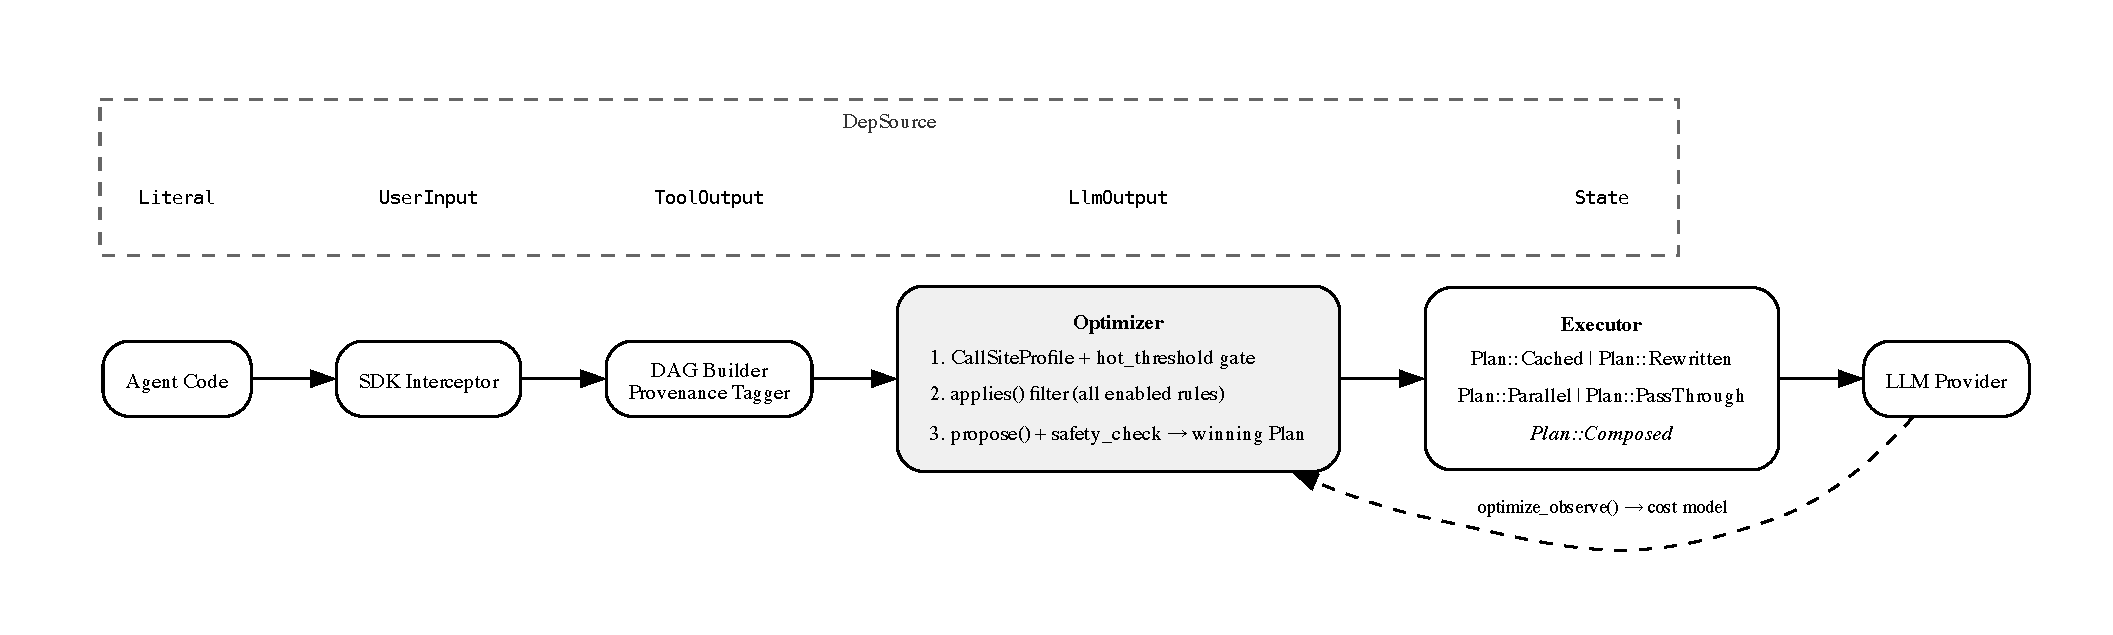
\includegraphics[width=\textwidth]{figures/fig1_architecture.pdf}
\caption{Agentc system architecture. Each intercepted call is lifted into a typed IR,
evaluated by the optimizer, and dispatched as one of four plan types:
\texttt{Plan::PassThrough}, \texttt{Plan::Rewritten}, \texttt{Plan::Composed}, or
\texttt{Plan::Parallel}. \texttt{Plan::Parallel} is a bookkeeping artifact recording
provenance-disjointness, not a scheduling directive; concurrent execution is realized
at the \texttt{parallel\_map} level independently of the optimizer
(Section~\ref{sec:decoupling}). Outcomes feed back into the per-call-site cost model
via \texttt{optimize\_observe()}.}
\label{fig:architecture}
\end{figure*}

\subsection{DAG IR and Provenance}

Each intercepted call is represented as a \texttt{Call} struct containing the model
identifier, message list, parameter block, tool configuration, a call-site identifier
derived from source location, and a trace identifier linking it to the enclosing
\texttt{@agentc.trace} span. Messages are the primary unit of transformation; rewrites
operate at the message level rather than the call structure.

Each message is annotated with a \texttt{DepSource} tag assigned by the Python
interceptor before execution reaches the optimizer. The five tag values are:
\texttt{Literal} (static string in source code), \texttt{UserInput} (content from a
user-facing input), \texttt{ToolOutput} (output from a tool invocation in this trace),
\texttt{LlmOutput} (output from a prior LLM call in this trace), and \texttt{State}
(written via \texttt{agentc.state\_write(key)}).

Provenance is tracked using an interning-based identity map maintained per execution
thread, mapping Python string objects to \texttt{DepSource} labels at construction
time. This design requires no developer annotations and supports heterogeneous message
assembly from multiple sources within a single prompt.

Provenance is a hard constraint in the rewrite system. Rules may read it but cannot
override it. In particular, messages tagged \texttt{UserInput} are never dropped by
any rule, regardless of attention score or state usage. \texttt{State}-tagged messages
carry their key identifier, enabling \texttt{StateDrop} to match them against the
current read window during optimization.

\subsection{Two-Gate Rule Pipeline}
\label{sec:twogatepipeline}

Each rewrite rule implements two methods: \texttt{applies()}, a lightweight filter,
and \texttt{propose()}, a full projection. \texttt{applies()} evaluates structural and
metadata preconditions, including prompt size thresholds, required field presence, and
whether a cheaper model route is available for the current model. \texttt{propose()}
performs the full optimization simulation, including attention scoring, message-drop
emulation, cost model lookup, and computation of projected savings in USD.

The planner invokes \texttt{applies()} for all enabled rules on every intercepted
call, and invokes \texttt{propose()} only for rules that pass this filter. This
separation ensures that expensive projection logic is never executed for rules that
cannot fire, avoiding per-call evaluation of full optimization logic and preventing
rule overhead from dominating end-to-end runtime cost.

Safety constraints are enforced as a separate stage from rule logic. The safety
checker enforces provenance-based invariants and overrides any proposal that violates
them, including any proposal that would remove a \texttt{UserInput}-tagged message.
This separation between proposal and safety check is intentional: rules can claim
arbitrary projected savings, but provenance invariants, including unconditional
preservation of \texttt{UserInput}-tagged messages and per-role retention floors, are
enforced by the planner, not by the rule. A rule cannot opt out of provenance
constraints by claiming a higher savings projection.

\begin{figure}[t]
\centering
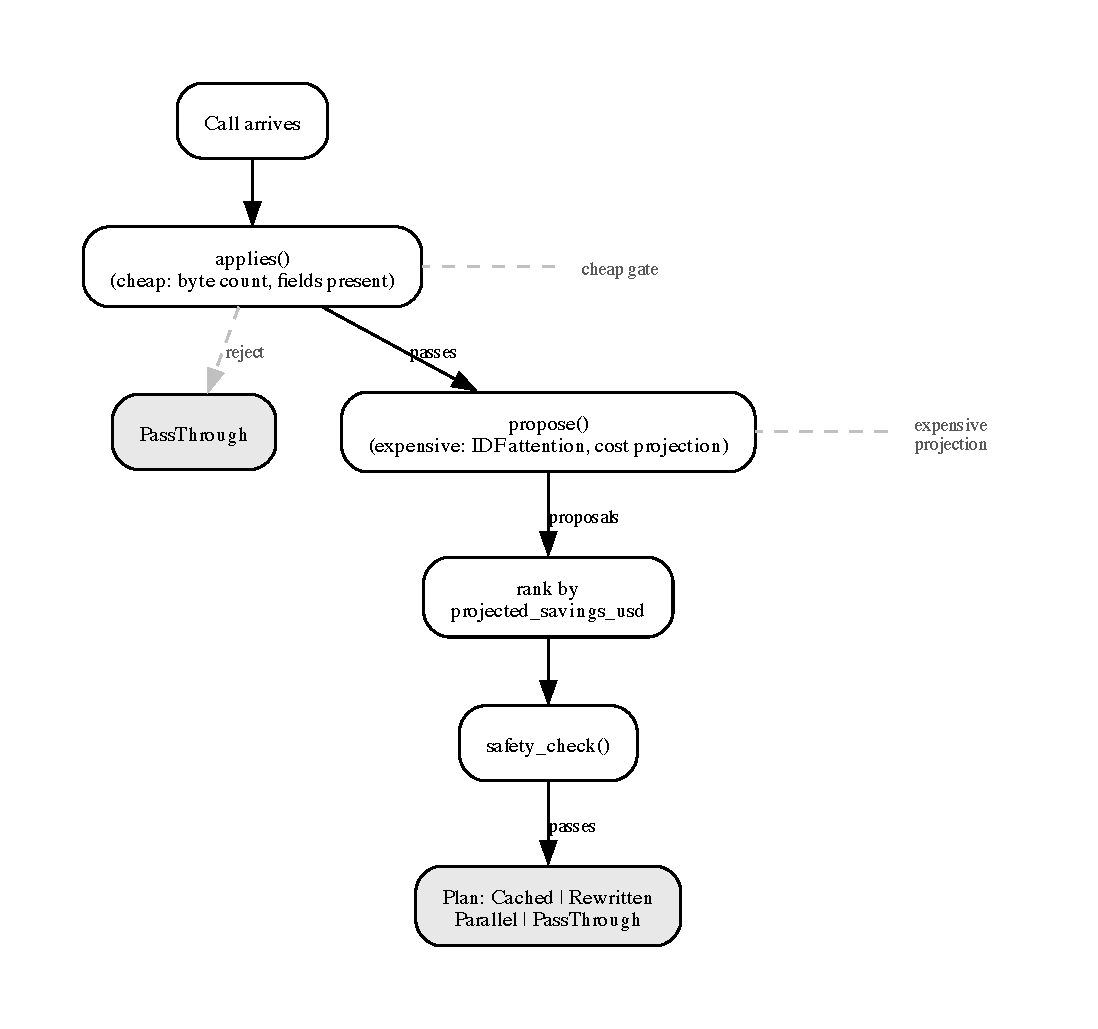
\includegraphics[width=\columnwidth]{figures/fig2_twogatepipeline.pdf}
\caption{Two-gate rule pipeline. \texttt{applies()} is a cheap structural filter;
\texttt{propose()} runs only for rules that pass, avoiding projection overhead on
calls where no rule can fire.}
\label{fig:twogates}
\end{figure}

\subsection{CompositionPlanner}
\label{sec:composition-planner}

An earlier first-match planner applied at most one rule per call, selecting the
highest-projected-savings proposal that passed safety checks. This policy leaves
compound savings unrealized when multiple rules could fire on the same call without
interfering. The current CompositionPlanner classifies rules by the cost driver they
target and combines rules with orthogonal cost drivers on the same call. The
classification is grounded in the observation that rules targeting non-overlapping
\texttt{Call} fields modify independent parts of the program state; their rewrites
commute and can be applied in a single pass without interference.

Table~\ref{tab:costdrivers} shows the full cost-driver taxonomy. Two rules compose
safely if and only if they have distinct \texttt{CostDriver} values, or they appear
on an explicit safe-pair allowlist. The allowlist covers cases where same-driver rules
are provably non-interfering: \texttt{(PromptDedup, ContextCompress)},
\texttt{(StateDrop, ContextCompress)}, and \texttt{(StateDrop, OutputBudget)}: in
each case the first rule removes a subset of messages and the second runs on the
remainder with no content overlap. Explicitly unsafe pairs are
\texttt{(StateDrop, PromptDedup)} and \texttt{(ContextCompress,
StructuredTruncation)}, where content mutations do not carry through the merge path.

\begin{table}[t]
\caption{Cost-driver taxonomy. Rules with distinct drivers modify non-overlapping
\texttt{Call} fields and compose safely; same-driver rules require explicit safe-pair
classification. The Structural driver (ParallelBranch) does not modify message content
but emits a provenance-disjointness certificate, signaling to the CompositionPlanner
that the paired branches are safe for concurrent handling.}
\label{tab:costdrivers}
\footnotesize
\begin{tabularx}{\columnwidth}{@{} l l X @{}}
\toprule
CostDriver & Rules & Field modified \\
\midrule
InputTokens  & CC, StateDrop, PromptDedup, StructTrunc & \texttt{messages} \\
OutputTokens & OutputBudget, DeadOutputTrunc & \texttt{max\_output\_tokens} \\
ModelPrice   & ModelDowngrade  & \texttt{model} \\
CallElim.    & CacheHit        & entire call \\
Structural   & ParallelBranch  & trace topology (disjointness cert.) \\
\bottomrule
\end{tabularx}
\end{table}

The CompositionPlanner selects a compatible set of proposals and applies them in
dependency order: StateDrop~$\rightarrow$~PromptDedup~$\rightarrow$
ContextCompress~$\rightarrow$~StructuredTruncation~$\rightarrow$
OutputBudget~$\rightarrow$~DeadOutputTruncation~$\rightarrow$
ModelDowngrade~$\rightarrow$~PrefixAlign. \texttt{CacheHit} (CallElimination) is
always applied solo; if selected, no other rule joins. Composed plans are recorded as
\texttt{Plan::Composed}, carrying a \texttt{Vec<RuleApplication>} with per-rule
projected savings and cost-driver attribution alongside \texttt{net\_savings\_usd}.
\texttt{Plan::Rewritten} records remain unchanged for solo-rule plans, preserving
attribution semantics of the earlier planner. \texttt{AGENTC\_COMPOSE=0} forces
first-match mode for regression testing.

The full planner, incorporating the hot-site gate, the two-gate pipeline, and the
CompositionPlanner, is shown in Algorithm~\ref{alg:planner}.

\begin{algorithm}
\caption{Agentc planner}
\label{alg:planner}
\begin{algorithmic}[1]
\If{optimizer disabled}
    \State \Return \texttt{Plan::PassThrough}
\EndIf
\State Load \texttt{CallSiteProfile} for current call site
\If{$\texttt{profile.n\_observations} < \texttt{hot\_threshold}$}
    \State \Return \texttt{Plan::PassThrough} \Comment{JIT gate: cold sites observe, hot sites optimize}
\EndIf
\State $\textit{applicable} \leftarrow \{r \in \textit{rules} \mid r.\texttt{applies}(\textit{call}, \textit{profile})\}$
\State $\textit{proposals} \leftarrow \bigcup_{r \in \textit{applicable}} r.\texttt{propose}(\textit{call}, \textit{profile})$
\State Sort $\textit{proposals}$ by $\texttt{projected\_savings\_usd}$ descending
\If{$\exists\, p \in \textit{proposals}$ s.t. $p.\texttt{driver} = \texttt{CallElimination}$}
    \State \Return first such $p.\texttt{plan}$ \Comment{CacheHit always solo}
\EndIf
\State $\textit{selected} \leftarrow [\;]$
\For{each $p \in \textit{proposals}$}
    \If{$p$ is safe w.r.t.\ all $s \in \textit{selected}$}
        \State Append $p$ to $\textit{selected}$
    \EndIf
\EndFor
\For{each $p \in \textit{selected}$}
    \If{$\neg$\texttt{safety\_check}($p$, \textit{call})}
        \State Remove $p$ from $\textit{selected}$
    \EndIf
\EndFor
\If{$|\textit{selected}| > 1$}
    \State Apply in dependency order
    \State \Return \texttt{Plan::Composed}(\textit{selected})
\ElsIf{$|\textit{selected}| = 1$}
    \State \Return \texttt{Plan::Rewritten}(\textit{selected}[0])
\Else
    \State \Return \texttt{Plan::PassThrough}
\EndIf
\end{algorithmic}
\end{algorithm}

\subsection{Cost Model}

Agentc maintains a \texttt{CallSiteProfile} for each call site, keyed by an
identifier derived from source location. Each profile tracks Welford-style streaming
statistics over observed outcomes, including mean and variance of per-call cost in
USD, input token count, output token count, and latency. Profiles are persisted in an
embedded SQLite store and updated after every dispatched call via
\texttt{optimize\_observe()}.

Rules do not fire on cold call sites. A configurable \texttt{hot\_threshold} (default:
3 observations) gates rule evaluation: calls to sites with fewer than
\texttt{hot\_threshold} observations return \texttt{Plan::PassThrough} and are used
only to update the corresponding profile. This cold-to-hot transition is the defining
characteristic of the JIT analogy: a call site begins in an observing state and
graduates to an optimizing state once the cost model holds sufficient data to project
savings reliably.

This gating mechanism is necessary because \texttt{propose()} computes projected
savings as a function of \texttt{profile.cost\_usd.mean}. On under-observed call
sites, this estimate is based on a small number of samples and produces high-variance
or degenerate projections, leading to unstable optimization decisions if used
prematurely.

In practice, this introduces a minimum viable experiment size. During development,
pilot runs at $n$=3 showed uniformly zero measured savings across all rule
configurations. This was expected: with \texttt{hot\_threshold}=3 and a single active
call site per agent, the optimizer correctly suppressed all rule evaluation due to
insufficient observations. As a result, experimental design must ensure that $n$
exceeds the product of \texttt{hot\_threshold} and the number of distinct call sites
in the agent. This constraint directly informs the benchmark construction in
Section~\ref{sec:methodology}.

\subsection{IDF Attention Proxy}

\texttt{ContextCompress} requires a per-message score estimating how much each message
contributes to the current call output. Internal model attention is not accessible
prior to inference, so Agentc uses a lightweight proxy: IDF-weighted token overlap
between each message and a \textit{salient signal} derived from the current call.

IDF weights are computed over the prompt's message set using add-1 smoothing. Tokens
appearing in many messages receive low weight, while tokens that are discriminative to
a small subset of messages receive higher weight. The resulting score is computed as a
normalized weighted overlap between message tokens and the salient signal. Messages
with scores below a configurable threshold are candidates for removal, subject to the
retention constraints described in Section~\ref{sec:rules}.

The salient signal is defined in \texttt{\_salient\_signal()} in
\path{python/agentc/_attention.py}. For single-turn and question-answering workloads,
the signal is the current call's last \texttt{role=user} message, which represents
the query against which contextual relevance is measured. For multi-turn agents
without fresh user input, the signal falls back to tokens derived from prior calls in
the same trace.

This design is critical to correctness. An earlier implementation defined the salient
signal as the union of prior-trace tokens and the current user message. In workloads
where a single \texttt{@agentc.trace} spans multiple independent tasks, prior-task
tokens accumulated across iterations, causing irrelevant overlap between unrelated
prompts. As a result, distractor messages frequently exceeded the drop threshold, even
when semantically unrelated to the current query. Under this configuration,
ContextCompress fired on only a small fraction of calls, yielding negligible savings.
After restricting the salient signal to the current call's last user message, the fire
rate increased to 87--95\% across configurations on the canonical $n$=300 fixture,
with 34\% input-token savings (Section~\ref{sec:eval-cc}). This demonstrates that
attention proxies operating over trace-level state must explicitly scope relevance to
the current task to avoid cross-task contamination.

\subsection{Execution-Optimizer Decoupling}
\label{sec:decoupling}

Agentc separates logical optimization from physical execution. The optimizer
produces a typed plan, including \texttt{Plan::PassThrough}, \texttt{Plan::Rewritten},
\texttt{Plan::Composed}, or \texttt{Plan::Parallel}, and hands it to a
dispatcher that is independent of the optimizer's rule evaluation pipeline. For
concurrent workloads, actual parallel dispatch is realized at the
\texttt{agentc.parallel\_map} level via a \texttt{ThreadPoolExecutor} that runs
the agent callback for each input item in parallel. The optimizer never manages
threads or synchronization primitives; it observes the calls those threads emit
and evaluates rules on each one independently.

This has three consequences. First, the optimizer cannot introduce race
conditions: it holds no shared mutable state across concurrent calls. Second,
\texttt{Plan::Parallel}, emitted by the ParallelBranch rule when a disjointness
certificate is produced, is a bookkeeping artifact, not a scheduling directive.
It records that the optimizer verified the paired calls are provenance-disjoint,
enabling the CompositionPlanner to confirm that messages produced by those branches
remain provenance-safe before they reach the next serial node. Third,
\texttt{dispatch\_sync} falls back to the original call path when no rewrite
applies; if the optimizer ever misidentifies a branch, the agent's core logic
executes unperturbed. Structural awareness without execution interference is a
design invariant, not a fallback.

Each major design decision in Agentc is motivated by a specific failure mode it
prevents. Provenance enforcement prevents any rule from silently dropping
\texttt{UserInput}-tagged messages regardless of projected savings: a rule cannot
opt out of this constraint by claiming a higher projection. Message-level granularity
for ContextCompress prevents token-level scoring from damaging supporting passages:
on HotpotQA-distractor, token-level scoring (LLMLingua-2) breaks 17 tasks the
baseline solves while Agentc breaks zero. Structure-sensitive preconditions prevent
compression where no structural signal exists: Agentc abstains on natural Wikipedia
prose (BF=0, FB=0) and on an unseen cold agent (support\_qa, 3-message prompts),
producing no savings and no regressions in both cases. The CompositionPlanner's
cost-driver orthogonality gate composes CC and OB without accuracy degradation on
composition\_qa: both CC+OB first-match and CC+OB composition achieve $+$14\,pp
($p$=0.0156). The read-window model for StateDrop prevents removing state that is
still consumed: when all state keys are present in \texttt{window\_state\_reads},
StateDrop fires 0 of 320 times across 320 measurement calls. Shared-baseline
ablation with input-token attribution prevents stochastic output variance from being
misread as rule effect: a single StateDrop trial at temperature~1 shows $-$7.0\% cost
despite a deterministic $+$6.7\% input-token reduction, rendering cost alone
uninterpretable. The evaluation in Section~\ref{sec:eval} is organized to present
each of these failure modes and their corresponding proofs.

\section{Rewrite Rules}
\label{sec:rules}

Agentc ships nine rewrite rules. Table~\ref{tab:rules} summarizes each rule's
\texttt{applies()} trigger and cost driver. Three rules are empirically validated in
isolation (Section~\ref{sec:eval}); two additional rules are validated through
composition experiments (Section~\ref{sec:eval-composition}); two are characterized
mechanistically; and two are descoped pending dedicated evaluation fixtures.

\textbf{ContextCompress.} \texttt{applies()} passes when the prompt exceeds 8,192
bytes and per-message attention scores are present in the call metadata.
\texttt{propose()} drops messages with IDF-weighted attention scores at or below 0.10,
provided at least 30\% of messages fall below this threshold. Removal is subject to a
retention floor of 50\% of original messages, per-role minimum retention, and
unconditional preservation of all \texttt{UserInput}-tagged messages. Compression is
extractive; no auxiliary LLM call is issued because its cost would exceed expected
savings in the targeted regime. Projected savings are estimated as
\texttt{cost\_usd.mean} multiplied by the fraction of messages removed. This rule
operates at message granularity, not token granularity, which is the key distinction
from LLMLingua-style methods (Section~\ref{sec:eval-llmlingua}).

\textbf{ModelDowngrade.} \texttt{applies()} passes when the call site is hot and a
cheaper model route is configured for the current model. Supported mappings are
\texttt{gpt-4o} $\rightarrow$ \texttt{gpt-4o-mini} and \texttt{gpt-4-turbo}
$\rightarrow$ \texttt{gpt-4o-mini}. \texttt{propose()} checks a per-call-site
accuracy constraint derived from the observed accuracy distribution of the shadow
sampler; proposals exceeding the allowable regression are rejected. Otherwise, savings
are computed from the difference in per-token pricing across model tiers. This rule
reduces cost without affecting input token counts.

\textbf{StateDrop.} \texttt{applies()} passes when \texttt{parameters.extra} contains
both \texttt{message\_deps} (per-message \texttt{DepSource} annotations) and
\texttt{window\_state\_reads} (state keys read since the previous LLM call in the
trace). In this context, \texttt{propose()} removes messages of type
\texttt{DepSource::State\{key\}} where \texttt{key} is not found in
\texttt{window\_state\_reads}, subject to a 50\% retention floor and system message
preservation. In iterative refinement workloads, earlier outputs accumulate as state
but are not re-consumed in later steps, making them safe to drop.

StateDrop's correctness rests on a runtime read-window model, not sound program
slicing. A \texttt{State}-tagged message with key $k$ is removable iff $k$ is absent
from the per-call \texttt{window\_state\_reads} set populated by
\texttt{agentc.state\_read}. This is conservative runtime pruning informed by
classical liveness
analysis~\cite{allen1976dataflow,weiser1981slicing,tip1995survey}, not
dependency-graph slicing over a static program. The 50\% retention floor and
unconditional system-message preservation provide additional defensive bounds:
StateDrop will never empty the message list, and the read window alone never decides
removal: the floor and provenance constraints override the rule.

\textbf{PromptDedup.} \texttt{applies()} passes when the prompt contains multiple
messages with near-duplicate token n-gram content. \texttt{propose()} identifies
near-duplicate message segments using independent per-call IDF and removes or shortens
redundant messages while preserving unique content. CostDriver: InputTokens. Validated
as a composition partner in Section~\ref{sec:eval-composition}.

\textbf{OutputBudget.} \texttt{applies()} passes when the call site has no existing
\texttt{max\_tokens} cap and has a measured output token p99 in the call site profile.
\texttt{propose()} sets \texttt{max\_output\_tokens} to the call site's p99 output
token count, capping runaway generation on call sites with consistently short outputs.
CostDriver: OutputTokens. Validated in the planner ablation
(Section~\ref{sec:eval-composition}).

\textbf{StructuredTruncation.} \texttt{applies()} passes when a message contains
structured JSON tool output and at least one field is unreferenced in downstream
messages (detected via field-name token presence in follow-on messages).
\texttt{propose()} projects out unreferenced JSON fields, passing only fields
referenced by later calls. This is the direct analog of projection pushdown in query
optimization. CostDriver: InputTokens. \textit{Characterized mechanistically; no
end-to-end benchmark result in this paper.}

\textbf{DeadOutputTruncation.} \texttt{applies()} passes when a call site's prior
outputs were historically unreferenced in subsequent messages. \texttt{propose()} sets
an aggressive \texttt{max\_output\_tokens} cap. CostDriver: OutputTokens.

Dead-output detection uses a token-overlap check between the step-$n$ output and
the step-$(n+1)$ input. An earlier implementation used a minimum token length of
3 characters, which admitted English stopwords (``the'', ``and'') as overlap
tokens; this caused the detector to always find overlap and never classify any
output as dead, producing a 0\% fire rate regardless of content. The fix replaces
the shared tokenizer with a dedicated \texttt{\_tokenize\_dead()} function using a
6-character minimum, which filters stopwords while retaining discriminative domain
tokens. DeadOutputTruncation fires correctly after this change. Firing remains
data-dependent: when step-$n$ reasoning reuses vocabulary that also appears in
step-$(n+1)$ inputs (common in document-heavy tasks), the detector correctly
abstains. \textit{No end-to-end benchmark result in this paper; characterized
mechanistically.}

\textbf{CacheHit.} \texttt{applies()} passes when the call site profile has at least
one observation and the memoization layer returns a cache hit on the canonical form of
the call. Exact matches are served directly; approximate matches require a similarity
score $\geq 0.95$ under the LSH index. CacheHit bridges
\texttt{@agentc.memoize}-decorated and non-decorated callers using a shared cache
namespace. CostDriver: CallElimination; always applied solo.

CacheHit requires a two-run approach by construction. Run~1 seeds the cache:
\texttt{optimize\_observe()} enqueues a cache insert in the per-process DB
(\texttt{active/pid-XXXX.db}) on every pass-through plan. \texttt{agentc.shutdown()}
then merges the per-process DB into \texttt{traces.db}. Run~2 finds the entries:
\texttt{applies()} queries \texttt{traces.db} and, on a hit, \texttt{\_decode\_cached\_openai}
reconstructs the response from stored content. Parameters are canonicalized via a
normalized serialization that omits empty fields (e.g., \texttt{stop:~[]}) to
ensure run-1 keys and run-2 lookups hash identically. Validated on
\texttt{batch\_classifier} (2 unique prompts $\times$ 10 repetitions $=$ 20 tasks):
run~2 returns \texttt{plan\_kind=cached} on all 20 tasks with 100\% accuracy
preserved (Section~\ref{sec:eval-cachehit}).

\textbf{ParallelBranch.} \texttt{applies()} passes when
\texttt{parameters.extra.\allowbreak parallel\_peer} is set and the
\texttt{input\_deps} of paired calls are disjoint under \texttt{DepSource}
annotations. \texttt{propose()} emits a disjointness certificate and a
\texttt{Plan::Parallel} record. Actual concurrent execution is realized by
\texttt{agentc.parallel\_map}'s \texttt{ThreadPoolExecutor}, which runs the agent
callback for each item in parallel independently of the optimizer; the optimizer
is never on the thread-dispatch path. \texttt{Plan::Parallel} is therefore a
bookkeeping artifact: it records that the optimizer verified the paired calls are
provenance-disjoint, enabling the CompositionPlanner to confirm that messages
produced by those branches are safe to merge at the next serial node. In the
current \texttt{dispatch\_sync} path, \texttt{Plan::Parallel} degrades to the
original call, which would have executed regardless; the disjointness certificate
and audit record are preserved for downstream analysis and future async executor
backends (Section~\ref{sec:futurework}).

\begin{table}[t]
\caption{The nine Agentc rewrite rules and their cost drivers.}
\label{tab:rules}
\footnotesize
\begin{tabularx}{\columnwidth}{@{} l X l @{}}
\toprule
Rule & \texttt{applies()} trigger & CostDriver \\
\midrule
ContextCompress  & prompt $>$8\,KB, attention scores present       & InputTokens \\
ModelDowngrade   & hot call site, cheaper model route configured   & ModelPrice \\
StateDrop        & \texttt{message\_deps} and \texttt{window\_state\_reads} present & InputTokens \\
PromptDedup      & near-duplicate messages detected                & InputTokens \\
OutputBudget     & no \texttt{max\_tokens} cap, p99 in profile     & OutputTokens \\
StructTrunc      & JSON tool output with unreferenced fields       & InputTokens \\
DeadOutputTrunc  & call site outputs historically unreferenced     & OutputTokens \\
CacheHit         & call site observed, cache hit                   & CallElim. \\
ParallelBranch   & \texttt{parallel\_peer} set, disjoint \texttt{input\_deps} & Structural \\
\bottomrule
\end{tabularx}
\end{table}

\section{Methodology}
\label{sec:methodology}

Evaluating an optimization runtime against stochastic LLM outputs requires care.
Output token counts vary across calls with identical prompts, and this variance can
dominate cost measurements: a rule that deterministically reduces input tokens by
6.7\% can appear to increase total cost by 7\% in a single trial if output tokens
increase due to sampling noise. Standard A/B evaluation is insufficient because
treatment modifies the prompt and therefore changes the output distribution. This
section describes the methodological choices that enable attribution of rule-level
effects.

\textbf{Documented failure modes.} The methodology described here is grounded in
three failure modes encountered during development, each of which invalidated an
earlier result set. First, cross-configuration optimizer-state contamination: when
multiple ablation configurations shared a single \texttt{traces.db}, the cost model
trained on one configuration's call history influenced another's rewrite decisions,
inflating CC and SD savings by conflating learning signals across configurations. Fix:
per-configuration isolated optimizer state with separate \texttt{traces.db},
\texttt{optimizer\_audit.db}, and \texttt{cost\_model.db} per run. Second, cold-start
cost model effects: ModelDowngrade's shadow-sampler accuracy guard reads the empirical
accuracy distribution from the cost model; on a cold-start run it effectively has no
data, so the guard defaults to permissive, causing over-downgrading and inflating MD
savings from the validated 11.4\%~(Section~\ref{sec:eval-md}) to a spurious 35.3\%. Fix: per-configuration warmup
($W$ tasks) that populates the cost model before measurement begins. Third, cross-run
baseline variance: a 37.8\% swing in baseline cost between two runs on identical
prompts (fresh cold-start run at \$136.19\,mUSD vs.\ warm shared-baseline at
\$84.70\,mUSD) makes cross-run cost attribution unreliable for rules that do not
affect input tokens. Fix: within-run input-token isolation as the authoritative
attribution signal. Section~\ref{sec:eval} demonstrates each failure mode and its
corresponding fix.

\subsection{Purpose-Built Workloads}

Rewrite rules fire only when their \texttt{applies()} preconditions are met. An
initial evaluation across four generic agents: a multi-agent researcher, a
SWE-bench planner, a RAG summarizer, and a GAIA router, produced near-zero
measured savings across all configurations, because these workloads did not reliably
trigger rule activation. Generic benchmarks are therefore not sufficient to evaluate
rule-level optimizations.

Each validated rule is evaluated on a purpose-built workload: a fixture and agent
constructed to reliably trigger the rule's \texttt{applies()} conditions, with prompt
structure designed around activation constraints. Importantly, these workloads are not
synthetic in data origin: \texttt{long\_context\_qa.json} is constructed from
Wikipedia passages drawn from the HotpotQA corpus, composed into multi-paragraph tasks
to reliably exceed the 8,192-byte activation threshold. The difference from standard
HotpotQA is composition, not source data. To reduce concern about regime-specific
behavior, each workload is additionally evaluated on a real-world corpus near the
activation boundary, as described in Section~\ref{sec:eval-hotpot}.

\subsection{Shared-Baseline Ablation}

Each agent is executed once with optimization disabled to collect a baseline
\texttt{RunStats} object. This baseline is reused across 11 configurations:
\textit{all-on}, five \textit{rule-off} variants, and five \textit{rule-only}
variants. Because all configurations share the same baseline, inter-run LLM variance
does not affect comparisons.

The resulting 11-configuration matrix enables per-rule attribution. A valid rule
should show consistent effects in configurations where it is active (\textit{all-on}
and \textit{rule-only}) and near-zero effect in its corresponding \textit{rule-off}
configuration. While this design reduces reliance on cross-run hypothesis testing, it
does not eliminate variance; it instead localizes comparison to
configuration-conditioned deltas.

\subsection{Input-Token Attribution}

Cost savings combine input and output token components. Output tokens are stochastic,
and therefore confound cost measurements across identical prompts. Input-token changes
are fully determined by the rewritten prompt and are deterministic conditional on the
rule output.

We therefore report both metrics for all experiments. When cost and input-token
savings track each other, savings are attributable to prompt reduction. When cost
savings are nonzero but input-token savings are zero, observed effects are attributable
to output-token sampling variance. Table~\ref{tab:attribution} illustrates this
distinction using StateDrop: a single trial at temperature 1 produces a $-$7.0\% cost
change despite a stable $+$6.7\% input-token reduction, while a temperature-0 trial
produces $+$1.9\% cost change with the same input-token reduction. Input-token
measurements remain stable across conditions, while cost measurements vary due to
decoding stochasticity.

\begin{table}[t]
\caption{Input-token savings as an attribution signal. Temperature 1 introduces
decoding variance, while temperature 0 isolates deterministic behavior. StateDrop
produces a consistent 6.7\% input-token reduction across both regimes.}
\label{tab:attribution}
\small
\begin{tabular}{lrr}
\toprule
Configuration & Cost $\Delta$ & Input-tok $\Delta$ \\
\midrule
StateDrop, temp=1, single trial  & $-$7.0\% & $+$6.7\% \\
StateDrop, temp=0                & $+$1.9\% & $+$6.7\% \\
ContextCompress-only             & $+$34.8\% & $+$34.9\% \\
ParallelBranch-only              & $0.0\%$  & $0.0\%$ \\
\bottomrule
\end{tabular}
\end{table}

For accuracy comparisons where per-task pass/fail outputs are available, we report
McNemar's exact test on discordant pairs. McNemar tests whether baseline-pass /
treatment-fail and baseline-fail / treatment-pass counts are symmetric; failure to
reject indicates that the optimization does not systematically degrade accuracy on
tasks the baseline solved. The exact binomial formulation is used throughout
(statsmodels \texttt{exact=True}), which is more conservative and appropriate than the
chi-squared approximation for small discordant-pair counts. Bootstrap confidence
intervals are computed by resampling task indices with replacement (5{,}000
iterations, percentile method).

\section{Evaluation}
\label{sec:eval}

All experiments use the shared-baseline ablation design described in
Section~\ref{sec:methodology}. Agents are executed in isolated subprocesses via
\texttt{agentc record}. Each configuration is run once with
\texttt{AGENTC\_OPTIMIZE=0} to establish a shared baseline and once per ablation
configuration with \texttt{AGENTC\_OPTIMIZE=1}. Standard errors on accuracy are
binomial and computed from the baseline pass rate; we report them alongside all
accuracy deltas. Total API spend across all reported experiments was under \$25
across OpenAI, Anthropic, and Together AI.

Table~\ref{tab:summary} summarizes results across all evaluated agents and providers;
the remainder of this section details each.

\begin{table*}[t]
\caption{Agentc across seven agent workloads spanning three distinct cost drivers,
three real agents, one unseen cold agent, and three model providers.
All real-agent accuracy deltas are not statistically significant.
Purpose-built workloads validate rule isolation;
real and unseen agents validate generalization. Rule specialization by workload class
is visible in the dominant-rule column: long-context agents are CC-dominated;
state-accumulating agents are SD-dominated.}
\label{tab:summary}
\footnotesize
\begin{tabularx}{\textwidth}{@{} l l l r r r r @{}}
\toprule
Agent & Type & Primary rule & Cost $\Delta$ & Tok $\Delta$ & Acc $\Delta$ & McNemar $p$ \\
\midrule
long\_context\_qa   & purpose-built QA      & ContextCompress      & 33.9\% & 34.0\% & $<$1\,pp (ns) & --- \\
gaia\_router        & purpose-built routing & ModelDowngrade       & 11.4\%$^\dagger$ &  0.0\% & $-$3.9\,pp (ns, $p$=0.18) & --- \\
iterative\_refiner  & purpose-built state   & StateDrop            & $\sim$4--6\,pp (within-run)$^\ddagger$ & see \S\ref{sec:eval-sd} & $<$1\,pp SD-neutral & --- \\
\midrule
autogen\_bridge     & real agent (Llama\,3.3-70B)  & CC             & ---$^\S$ & 38.5\% & $-$3.0\,pp (ns, $p$=0.07) & 0.07 \\
research\_planner   & real agent            & CC~+~StateDrop       & 25.8\% & 33.0\% & --- & --- \\
debug\_agent        & real agent            & StateDrop            &  8.3\% & 16.8\% & --- & --- \\
\midrule
support\_qa         & unseen cold agent     & correct abstain      & $\sim$0\% & $\sim$0\% & 0.0\,pp & 1.000 \\
\bottomrule
\end{tabularx}
\footnotesize{$\dagger$MD-only cost savings: 11.23\,mUSD / 98.91\,mUSD baseline = 11.4\%. All input-tok deltas $\approx$0 (ModelPrice driver).}\\
\footnotesize{$\ddagger$Within-run SD contribution: SD-only $\sim$6.1\% vs.\ SD-off $\sim$2.1\%; other configs show small ns deltas attributable to non-SD rules active in those configs.}\\
\footnotesize{$\S$Together AI cost model not in Agentc pricing table; input-token savings (38.5\%) shown in Tok column.}
\end{table*}

Optimizer overhead, measured across 1{,}818 plan decisions captured in the
\texttt{plan\_audit} table, has median 76\,\textmu s on the pass-through path (the
common case when no rule fires) and median 120\,\textmu s on the rewrite path. The
pass-through distribution is bimodal: cold-start cost-model loads on first call-site
invocation account for the p99 = 21\,ms tail, while warm-state pass-through stays
below 100\,\textmu s. The rewrite path is tighter (p95 = 0.35\,ms, p99 = 1.2\,ms).
Overhead scales sub-linearly with context length: p50 grows from 0.33\,ms to
0.71\,ms over a 16$\times$ size range (4\,KB to 64\,KB). All overhead is at least
three orders of magnitude below typical LLM round-trip latency. The flat overhead
profile under concurrency is attributable to the execution-optimizer decoupling
described in Section~\ref{sec:decoupling}: because the optimizer holds no shared
mutable state across concurrent calls and never manages threads, it does not become
a serialization point under parallel workloads.

\begin{figure}[t]
\centering
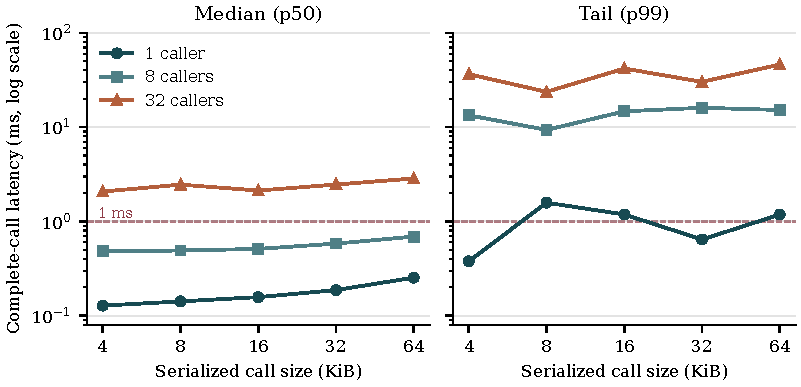
\includegraphics[width=\columnwidth]{figures/fig7_overhead_scaling.pdf}
\caption{Planner overhead scales sub-linearly with context length.
p50 grows from 0.33\,ms to 0.71\,ms over a 16$\times$ size range
(4\,KB to 64\,KB); p95 stays under 1.5\,ms throughout. The p99
spike at 8\,KB is a SQLite audit write, not IDF computation. All
overhead remains three orders of magnitude below typical LLM
round-trip latency.}
\label{fig:overhead}
\end{figure}

\begin{figure}[t]
\centering
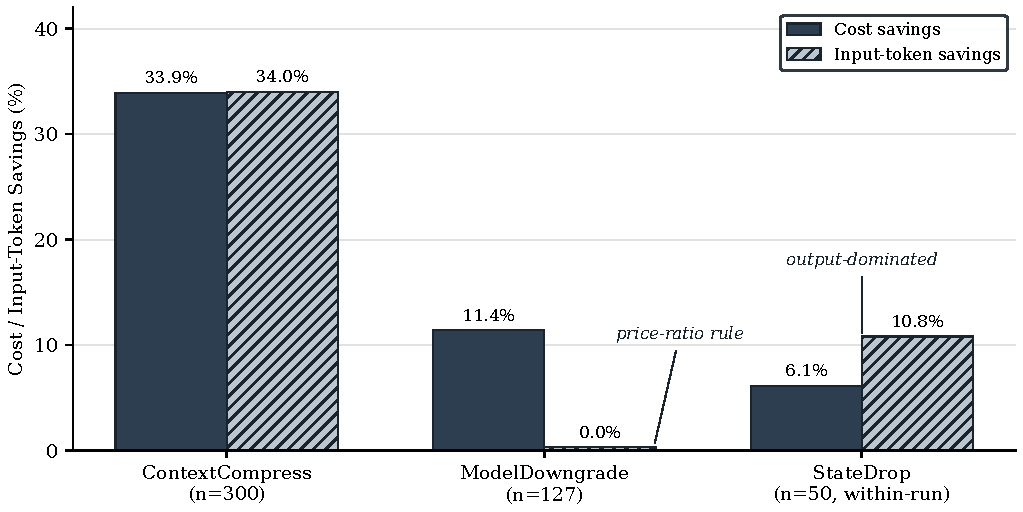
\includegraphics[width=\columnwidth]{figures/fig3_headline_savings.pdf}
\caption{Headline cost and input-token savings per validated rule ($n$=300 for
ContextCompress, $n$=127 for ModelDowngrade, $n$=50 within-run for StateDrop).
Cost and input-token columns track each other for ContextCompress (33.9\%/34.0\%)
and StateDrop (within-run, output-dominated), confirming deterministic attribution.
ModelDowngrade savings are structural: price per token, not token count (11.23\,mUSD
cost savings, 0\% input-token savings). StateDrop bar shows within-run contribution;
cross-run cost is confounded by baseline variance (Section~\ref{sec:eval-sd}).}
\label{fig:headline}
\end{figure}

\subsection{ContextCompress}
\label{sec:eval-cc}

\textbf{Setup.} \texttt{long\_context\_qa.json} contains 300 tasks constructed from
HotpotQA-distractor passages expanded to 20 paragraphs per task, producing prompts of
13--18\,KB (median 17\,KB). All tasks exceed the 8,192-byte activation threshold. The
agent is \path{bench/agents/long_context_qa.py} using \texttt{gpt-4o-mini} under
an 11-configuration ablation with per-configuration isolated optimizer state and
per-configuration warmup ($W$=30). Reported cost figures include OpenAI native prefix
caching, which is active by default; ContextCompress savings are measured in addition
to any prefix-cache effects.

\textbf{Results.} ContextCompress fires on 261 to 286 of 300 calls across
configurations (87 to 95\%), varying by which other rules are active; CC-off
configurations show 0 of 300 fires, confirming the precondition is stable. The full
isolation matrix is shown in Table~\ref{tab:cc-matrix}. Configurations containing
ContextCompress reduce cost and input tokens by approximately 34\%, while
configurations without it show 0.0\% cost and input-token change. This consistent
tracking supports attribution of savings to input-token reduction. All 11
configurations pass McNemar exact test with $p \geq 0.39$, SE $\pm$2.8\,pp at
$n$=300, baseline pass rate 58.3\%; no configuration shows a statistically significant
accuracy change. CacheHit-off (36.9\%) and StateDrop-off (36.8\%) exceed all-on
(33.9\%) because the removed rule occasionally serves or rewrites a call before CC
evaluates it, slightly reducing CC's aggregate fire opportunity; the 0\% savings on
ContextCompress-off remains the definitive precondition check.

\begin{table}[t]
\caption{ContextCompress isolation matrix ($n$=300, \texttt{long\_context\_qa},
\texttt{gpt-4o-mini}, warmup-corrected). Top block: configurations where CC is
active. Bottom block: rule-only configurations. Bold rows are the key comparators.
SE: $\pm$2.8\,pp. All McNemar exact $p \geq 0.39$ (ns). Baseline pass rate 58.3\%.}
\label{tab:cc-matrix}
\small
\begin{tabular}{lrrr}
\toprule
Configuration & Cost $\Delta$ & Input-tok $\Delta$ & Acc $\Delta$ \\
\midrule
\textbf{all-on}                 & \textbf{33.9\%} & \textbf{34.0\%} & $+$0.3\,pp \\
CacheHit-off                    & 36.9\% & 37.1\% & $+$1.7\,pp \\
\textbf{ContextCompress-off}    & \textbf{0.0\%}  & \textbf{0.0\%}  & $+$0.0\,pp \\
ParallelBranch-off              & 34.3\% & 34.4\% & $+$0.0\,pp \\
ModelDowngrade-off              & 33.0\% & 33.1\% & $-$1.0\,pp \\
StateDrop-off                   & 36.8\% & 36.9\% & $+$1.3\,pp \\
\midrule
CacheHit-only                   & 0.0\%  & 0.0\%  & $+$0.0\,pp \\
\textbf{ContextCompress-only}   & \textbf{36.1\%} & \textbf{36.3\%} & $+$1.7\,pp \\
ParallelBranch-only             & 0.0\%  & 0.0\%  & $-$1.3\,pp \\
ModelDowngrade-only             & 0.0\%  & 0.0\%  & $+$0.3\,pp \\
StateDrop-only                  & 0.0\%  & 0.0\%  & $-$1.0\,pp \\
\bottomrule
\end{tabular}
\end{table}

\textbf{Provider generalization.} To confirm that rule behavior depends on message
structure rather than model internals, we replicate the CC-only configuration on two
additional providers ($n$=50 each). On
\texttt{meta\allowbreak-llama/Llama-3.3-70B-Instruct} via HuggingFace Inference API,
ContextCompress achieves 34\% input-token savings at a 98\% fire rate, within
1\,pp of the OpenAI baseline (34.0\%, 87--95\%) despite a different model family,
tokenizer, and pricing tier. On Anthropic (\texttt{claude-haiku-4-5}),
ContextCompress achieves 0\% savings: the Anthropic API concatenates multi-paragraph
context into a single user message, leaving no droppable message units. The rule
correctly abstains. These results confirm that ContextCompress is structurally
invariant when its precondition is met and correctly inactive when it is not
(Figure~\ref{fig:provider}).

\subsection{ModelDowngrade}
\label{sec:eval-md}

\textbf{Setup.} \texttt{gaia\_router.json} contains 127 tasks from the GAIA
validation set (text-only subset). The agent is \path{bench/agents/gaia_router.py}
using baseline model \texttt{gpt-4o} with a configured downgrade route
\texttt{gpt-4o}~$\rightarrow$~\texttt{gpt-4o-mini}, evaluated under the ablation of
11 configurations with per-configuration isolated optimizer state and per-configuration
warmup. Reported cost figures reflect OpenAI native prefix caching active by default;
ModelDowngrade savings are additional to any prefix-cache effects.

\textbf{Results.} The full isolation matrix is shown in Table~\ref{tab:md-matrix}.
ModelDowngrade-only achieves 11.4\% cost savings (11.23\,mUSD from 98.91\,mUSD
baseline), with MD firing on 25.6\% of calls in the MD-only configuration and on
32.7\% of calls in the all-on configuration. Input-token deltas remain approximately
zero across all configurations, as expected: ModelDowngrade affects price per token
rather than token count. All-on cost saving is 19.7\%. The accuracy delta for
ModelDowngrade-only is $-$3.9\,pp; McNemar exact $p$=0.18, BF=7/FB=2,
$n_{\mathrm{discordant}}$=9. The effect is directionally negative but not
statistically significant at $n$=127; we do not claim ModelDowngrade does not degrade
accuracy, only that the effect is not confirmed at this sample size.

On this routing fixture, only ModelDowngrade fires; all other rule-only
configurations (CacheHit-only, CC-only, SD-only, PB-only) show near-zero input-token
savings, with negative cost values (e.g., CC-only $-$3.4\%, SD-only $-$6.7\%)
reflecting output-token sampling variance around zero, not rule-driven effects.

The corrected cost savings reflect ModelDowngrade operating with its shadow-sampler
accuracy guard active. A warm cost model provides the accuracy guard with a reliable
empirical accuracy distribution to gate against. An earlier cold-start measurement
reflected the accuracy guard effectively disabled due to insufficient observations,
causing over-downgrading. The 11.4\% figure is the valid estimate with the safety
constraint active.

\begin{table}[t]
\caption{ModelDowngrade isolation matrix ($n$=127, \texttt{gaia\_router},
\texttt{gpt-4o}~$\rightarrow$~\texttt{gpt-4o-mini}, warmup-corrected). Top block:
rule-off configurations. Bottom block: rule-only configurations. Bold rows are the
key comparators. Input-token savings are structurally zero throughout. SE:
$\pm$3.0\,pp. Baseline pass rate 15.0\%. Negative cost savings for CC-only
and SD-only reflect output-token variance; input-tok savings are $\approx$0,
confirming no rule-driven effect.$^\dagger$}
\label{tab:md-matrix}
\small
\begin{tabular}{lrrrr}
\toprule
Configuration & Cost $\Delta$ & Input-tok $\Delta$ & Acc $\Delta$ & MD fires \\
\midrule
all-on                          & 19.7\% & $\approx$0\% & $-$1.6\,pp & 83 (32.7\%) \\
CacheHit-off                    & 22.6\% & $\approx$0\% & $-$3.9\,pp & 72 (28.3\%) \\
ContextCompress-off             & 28.1\% & $\approx$0\% & $-$1.6\,pp & 82 (32.3\%) \\
ParallelBranch-off              & 29.1\% & $\approx$0\% & $-$2.4\,pp & 83 (32.7\%) \\
\textbf{ModelDowngrade-off}     & \textbf{1.9\%} & $\approx$0\% & $-$0.8\,pp & 0 (0.0\%) \\
StateDrop-off                   & 31.2\% & $\approx$0\% & $-$3.9\,pp & 83 (32.7\%) \\
\midrule
CacheHit-only                   & $-$0.6\% & $\approx$0\% & $-$1.6\,pp & 0 (0.0\%) \\
ContextCompress-only$^\dagger$  & $-$3.4\% & $\approx$0\% & $+$1.6\,pp & 0 (0.0\%) \\
ParallelBranch-only             & 3.5\%  & $\approx$0\% & $-$0.8\,pp & 0 (0.0\%) \\
\textbf{ModelDowngrade-only}    & \textbf{11.4\%} & \textbf{$\approx$0\%} & $-$3.9\,pp ($p$=0.18, ns) & 65 (25.6\%) \\
StateDrop-only$^\dagger$        & $-$6.7\% & $\approx$0\% & $-$1.6\,pp & 0 (0.0\%) \\
\bottomrule
\end{tabular}
\footnotesize{$\dagger$CC and SD do not fire on this routing fixture (short prompts, no state-tagged messages). Negative cost values are output-token sampling variance around zero; input-tok savings $\approx$0 in all rows.}
\end{table}

\textbf{Provider generalization.} ModelDowngrade achieves 14.7\% cost reduction on
Anthropic (\texttt{claude-sonnet-4-5}~$\rightarrow$~\texttt{claude-haiku-4-5}, 20\%
fire rate, $n$=50) and 31.1\% on HuggingFace
Llama-3.3-70B~$\rightarrow$~Llama-3.1-8B (34\% fire rate, $n$=50). The Anthropic
accuracy delta of $+$4\,pp is a fixture artifact: exact-match scoring penalizes the
more verbose sonnet outputs even when answers are semantically correct; rule behavior
is correct. Savings magnitude varies by pricing tier; routing logic is
provider-agnostic.

\begin{figure}[t]
\centering
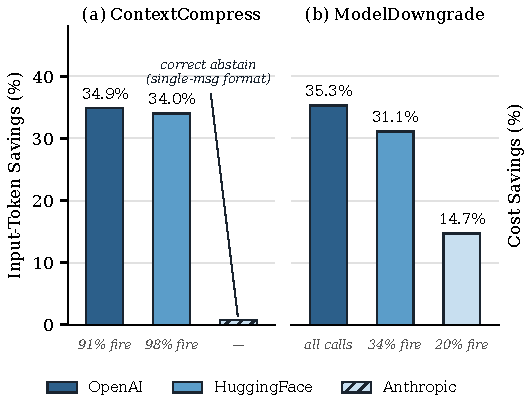
\includegraphics[width=\columnwidth]{figures/fig4_provider_generalization.pdf}
\caption{Provider generalization for ContextCompress (input-token savings) and
ModelDowngrade (cost savings) across OpenAI, HuggingFace Inference API
(Llama-3.3-70B), and Anthropic ($n$=50 each). CC savings are within 1\,pp
across OpenAI and HuggingFace despite different model families, tokenizers,
and pricing tiers. Anthropic CC achieves 0\% savings by correct
abstention: the Anthropic API concatenates multi-paragraph context into a
single user message, leaving no droppable message units. MD savings vary
by pricing tier as expected; routing logic is provider-agnostic.}
\label{fig:provider}
\end{figure}

\subsection{StateDrop}
\label{sec:eval-sd}

\textbf{Setup.} \texttt{bench/agents/iterative\_refiner.py} implements a 10-step
refinement chain. At each step, the prior revision is appended to the message list as
a \texttt{state\_write}-tagged message, while only the most recent revision is read
into the current call window. Older revisions accumulate as state-tagged messages
whose keys are absent from \texttt{window\_state\_reads}, making them eligible for
removal by StateDrop. The fixture contains 50 tasks, producing 500 LLM calls in
total. Model: \texttt{gpt-4o-mini}. All eleven ablation configurations completed under
the warmup-corrected harness (temperature=0 hardcoded in agent).

\textbf{Results.} The valid comparison for StateDrop is within-run isolation, not
cross-run absolute savings. Within a controlled run, StateDrop-off configurations
settle at approximately 2.1\% cost savings and 2.1\% input-token savings (reflecting
other active rules), while StateDrop-only recovers to approximately 6.1\% cost and
10.8\% input-token savings; StateDrop contributes roughly 4 to 5\,pp of cost savings
within a run. Input-token attribution confirms the mechanism: SD fires 177 to 187
calls per SD-enabled configuration and 0 calls on SD-off configurations.

\textbf{Accuracy.} StateDrop in isolation is accuracy-neutral (SD-only 0.0\,pp,
McNemar $p$=1.0). Multi-rule configurations show small deltas (e.g., all-on
$-$4.0\,pp) that are not statistically significant (all McNemar $p \geq 0.25$,
SE~$\pm$2.0\,pp, $n$=50, baseline 98\%); at this $n$ a $-$4.0\,pp delta is a
one-task swing.

A cross-run comparison of baseline costs reveals a 37.8\% cost difference between a
fresh cold-start run (\$136.19\,mUSD) and the warm shared-baseline run
(\$84.70\,mUSD) on identical prompts, while optimized costs remained stable across
both runs. This baseline swing is the cleanest empirical motivation for the
input-token attribution methodology (Section~\ref{sec:methodology}): when baseline
cost is confounded by JIT warm-up effects, within-run isolation using input-token
deltas provides a reliable attribution signal independent of cost measurement.

\begin{table}[t]
\caption{StateDrop contribution matrix ($n$=50, \texttt{iterative\_refiner},
\texttt{gpt-4o-mini}, warmup-corrected). Valid comparison is within-run isolation.
SD-only tok savings 10.8\%, SD-off tok savings 2.1\%; SD contributes $\sim$4--5\,pp
within a run. SD fires 177--187 calls per SD-enabled config, 0 on SD-off.
SD-only Acc $\Delta$=0.0\,pp confirms accuracy neutrality; non-zero deltas in
multi-rule configs are attributable to other active rules, all McNemar
$p \geq 0.25$ (ns). SE: $\pm$2.0--3.4\,pp.}
\label{tab:sd-matrix}
\small
\begin{tabular}{lrrr}
\toprule
Configuration & Cost $\Delta$ & Input-tok $\Delta$ & Acc $\Delta$ \\
\midrule
all-on                          & 7.6\%  & 12.0\%  & $-$4.0\,pp (ns) \\
CacheHit-off                    & 7.5\%  & 12.1\%  & $-$6.0\,pp (ns) \\
ContextCompress-off             & 7.3\%  & 11.8\%  & 0.0\,pp \\
ParallelBranch-off              & 7.5\%  & 11.6\%  & 0.0\,pp \\
ModelDowngrade-off              & 8.2\%  & 12.7\%  & $-$4.0\,pp (ns) \\
\textbf{StateDrop-off}          & \textbf{2.1\%}  & \textbf{2.1\%}  & $-$4.0\,pp (ns) \\
\midrule
CacheHit-only                   & 2.8\%  & 2.5\%   & 0.0\,pp \\
ContextCompress-only            & 2.3\%  & 2.1\%   & 0.0\,pp \\
ParallelBranch-only             & 0.9\%  & 0.7\%   & 0.0\,pp \\
ModelDowngrade-only             & 0.9\%  & 0.9\%   & 0.0\,pp \\
\textbf{StateDrop-only}         & \textbf{6.1\%}  & \textbf{10.8\%} & \textbf{0.0\,pp} \\
\bottomrule
\end{tabular}
\end{table}

\textbf{Precondition validation.}
To confirm that the read-window check is the mechanism rather than message count or
prompt length, we evaluate a modified \texttt{iterative\_refiner} variant
(\texttt{iterative\_refiner\_allread}) in which every prior revision IS included in
\texttt{window\_state\_reads}: all state keys are consumed in each step. Under the
warmup-corrected harness ($W$=30, $N$=32, isolated optimizer state), StateDrop fires
0 of 320 measurement calls. The standard \texttt{iterative\_refiner} fires on 36\%
of calls (116 of 320) under structurally identical conditions. The difference is
entirely determined by the read-window check: when no key is absent from
\texttt{window\_state\_reads}, no message is droppable by construction. The 36\% fire
rate in the standard variant is consistent with the 35.8\% measured in the $n$=50
warmup-corrected ablation, and lower than earlier cold-start estimates because the
cost model's accuracy guard requires warmup observations before becoming selective.
The precondition is the mechanism.

\subsection{ContextCompress on Real HotpotQA}
\label{sec:eval-hotpot}

\textbf{Setup.} We evaluate ContextCompress on the HotpotQA-distractor split ($n$=300,
\texttt{gpt-4o-mini}). Prompts are not length-expanded; median size is 6,940 bytes.
82 of 500 tasks exceed the 8,192-byte activation threshold (the first 300 are
evaluated). All 11 configurations completed under the warmup-corrected harness.

\textbf{Results.} ContextCompress fires 0--1 of 300 calls depending on configuration
(1 in CC-active configs, 0 in CC-inactive configs), producing negligible aggregate
savings. For prompts near the activation threshold, the rule correctly avoids
execution when projected savings do not exceed overhead. On fully activated workloads
(Section~\ref{sec:eval-cc}), the rule produces substantial reductions, indicating that
performance depends primarily on activation frequency. The correct abstention behavior
on near-boundary natural prompts is also documented in
Section~\ref{sec:eval-llmlingua}.

\begin{table}[t]
\caption{ContextCompress on HotpotQA-distractor ($n$=300, \texttt{gpt-4o-mini},
warmup-corrected, all 11 configs). Median prompt 6,940 bytes; 82 of 500 tasks exceed
the 8,192-byte activation gate (first 300 evaluated). CC fires 0--1 of 300 per
config, confirming correct abstention near the activation boundary. Baseline 57.3\%,
SE~$\pm$2.9\,pp. All McNemar $p \geq 0.18$ (ns).}
\label{tab:hotpot-matrix}
\small
\begin{tabular}{lrrrr}
\toprule
Configuration & Input-tok $\Delta$ & Acc $\Delta$ & McNemar $p$ & CC/300 \\
\midrule
\textbf{all-on}              & $+$0.19\% & $-$1.7\,pp & 0.27 & 1 \\
CacheHit-off                 & $+$0.19\% & $-$1.0\,pp & 0.61 & 1 \\
\textbf{ContextCompress-off} & $\phantom{+}$0.00\% & $+$0.7\,pp & 0.79 & 0 \\
ParallelBranch-off           & $+$0.19\% & $-$1.7\,pp & 0.30 & 1 \\
ModelDowngrade-off           & $+$0.19\% & $-$2.0\,pp & 0.21 & 1 \\
StateDrop-off                & $\phantom{+}$0.00\% & $-$1.3\,pp & 0.45 & 0 \\
\midrule
CacheHit-only                & $\phantom{+}$0.00\% & $-$0.3\,pp & 1.00 & 0 \\
\textbf{ContextCompress-only}& $+$0.19\% & $-$2.0\,pp & 0.18 & 1 \\
ParallelBranch-only          & $\phantom{+}$0.00\% & $-$1.0\,pp & 0.63 & 0 \\
ModelDowngrade-only          & $\phantom{+}$0.00\% & $-$1.0\,pp & 0.58 & 0 \\
StateDrop-only               & $\phantom{+}$0.00\% & $-$1.3\,pp & 0.45 & 0 \\
\bottomrule
\end{tabular}
\end{table}

\subsection{Oracle Compression Ceiling}
\label{sec:eval-oracle}

We evaluate an oracle compression strategy that removes all non-supporting paragraphs
using HotpotQA annotations, providing an upper bound on achievable compression. Oracle
compression reduces input tokens by 5.6$\times$ and cost by 82\%, while improving
exact-match accuracy from 57.0\% to 64.3\%. This indicates that distractor context is
actively harmful in this setting and establishes the upper bound that ContextCompress
approaches on fully activated workloads.

\begin{table}[t]
\caption{Oracle compression ceiling ($n$=300). All figures read directly from
\texttt{traces.db}; no values are derived.}
\label{tab:oracle}
\small
\begin{tabular}{lrrr}
\toprule
Configuration & EM & Cost (USD) & Avg input tok/call \\
\midrule
Baseline               & 57.0\% & \$0.0786 & 1,734 \\
ContextCompress active & 58.3\% & \$0.0784 & 1,730 \\
Oracle                 & 64.3\% & \$0.0145 &   309 \\
\bottomrule
\end{tabular}
\end{table}

\subsection{LLMLingua-2 Comparison}
\label{sec:eval-llmlingua}

\textbf{Setup.} We compare ContextCompress against LLMLingua-2~\cite{pan2024llmlingua2}
on two workloads that test different structural regimes. The first is
HotpotQA-distractor ($n$=100, \texttt{gpt-4o-mini}): each task contains 10 paragraphs,
2 supporting and 8 injected distractors with low unigram overlap to the question.
This fixture is favorable for IDF-weighted scoring by construction, as distractor
messages are identifiable at message granularity as low-attention units. The second is
a natural Wikipedia prose workload ($n$=39): each task contains 18 paragraphs from the
same Wikipedia article, all topically related to the subject, with no injected
distractors. LLMLingua-2 uses the \texttt{xlm-roberta-large} compression model
(300\,MB); Agentc uses its 28\,MB IDF proxy with zero auxiliary inference. All
McNemar tests use the exact binomial formulation.

\textbf{Results: distractor fixture.} Table~\ref{tab:llmlingua-distractor} shows
results on the distractor workload. Agentc improves accuracy from 68\% to 100\%
(McNemar exact $p=4.66\times10^{-10}$, BF=0, FB=32): it rescues all 32 tasks the
baseline fails while degrading none it solves. LLMLingua-2 achieves the same 53.1\%
token reduction but degrades accuracy from 68\% to 53\% ($p=0.0013$, BF=17, FB=2):
it breaks 17 tasks the baseline solves while recovering only 2.

The mechanism is granularity. ContextCompress operates at message granularity and
drops entire distractor messages whose IDF-weighted attention scores fall below
threshold. The 8 injected distractors, by construction, share few content words with
the question and are cleanly identified as low-attention messages. LLMLingua-2
operates at token granularity within messages; its token-level importance scoring
removes content from both distractor and supporting passages, damaging the answer
content in the supporting paragraphs (BF=17).

\begin{table}[t]
\caption{LLMLingua-2 vs.\ Agentc on HotpotQA-distractor ($n$=100).
McNemar exact (two-sided). Discordant pairs: Agentc BF=0/FB=32;
LLMLingua-2 BF=17/FB=2.}
\label{tab:llmlingua-distractor}
\footnotesize
\begin{tabularx}{\columnwidth}{@{} l r r r r r r @{}}
\toprule
Method & Acc & SE & $\Delta$pp & $p$ & Tok & OH \\
\midrule
Baseline    & 68.0\% & $\pm$4.7 & --- & --- & 0\% & 0\,ms \\
Agentc (CC) & 100.0\% & $\pm$0.0 & $+$32 & $4.66\!\times\!10^{-10}$ & 53\% & $<$1\,ms \\
LLMLingua-2 & 53.0\%  & $\pm$5.0 & $-$15 & 0.0013 & 53.1\% & 11{,}400\,ms \\
\bottomrule
\end{tabularx}
\end{table}

\textbf{Results: natural prose.} Table~\ref{tab:llmlingua-wikipedia} shows results on
the natural Wikipedia workload. Agentc abstains completely: BF=0, FB=0, $p=1.0$,
identical outcomes to baseline on all 39 tasks. The structural precondition for
ContextCompress, multi-message context with messages identifiable as low-attention
units, is absent when all 18 paragraphs are topically related. The rule correctly
declines to fire, producing zero overhead and zero savings. LLMLingua-2 compresses
53.5\% of tokens regardless of workload structure, achieves no statistically
significant benefit ($p=1.0$, FB=1), and imposes 13{,}678\,ms of CPU inference
overhead per task.

\begin{table}[t]
\caption{LLMLingua-2 vs.\ Agentc on natural Wikipedia prose ($n$=39).
Agentc abstains (BF=0, FB=0); LLMLingua-2 BF=0/FB=1.}
\label{tab:llmlingua-wikipedia}
\footnotesize
\begin{tabularx}{\columnwidth}{@{} l r r r r r r @{}}
\toprule
Method & Acc & SE & $\Delta$pp & $p$ & Tok & OH \\
\midrule
Baseline    & 94.9\% & $\pm$3.5 & --- & --- & 0\% & 0\,ms \\
Agentc (CC) & 94.9\% & $\pm$3.5 & 0.0 & 1.000 & 0\% & $<$1\,ms \\
LLMLingua-2 & 97.4\% & $\pm$2.5 & $+$2.6 & 1.000 & 53.5\% & 13{,}678\,ms \\
\bottomrule
\end{tabularx}
\end{table}

\textbf{Dual-regime interpretation.} The two results together establish a dual-regime
picture. On favorable structure, Agentc improves accuracy with statistical significance
while LLMLingua-2 significantly degrades it. On natural structure, Agentc correctly
abstains while LLMLingua-2 compresses indiscriminately with no benefit and 13.7\,s
overhead. The critical distinction is not which method achieves higher compression on
favorable workloads, since both achieve 53\%, but which method has a principled
precondition that governs when compression is applied. Agentc's abstention on natural
prose is correct behavior, not a failure; it reflects the structural precondition
working as designed.

\begin{figure*}[t]
\centering
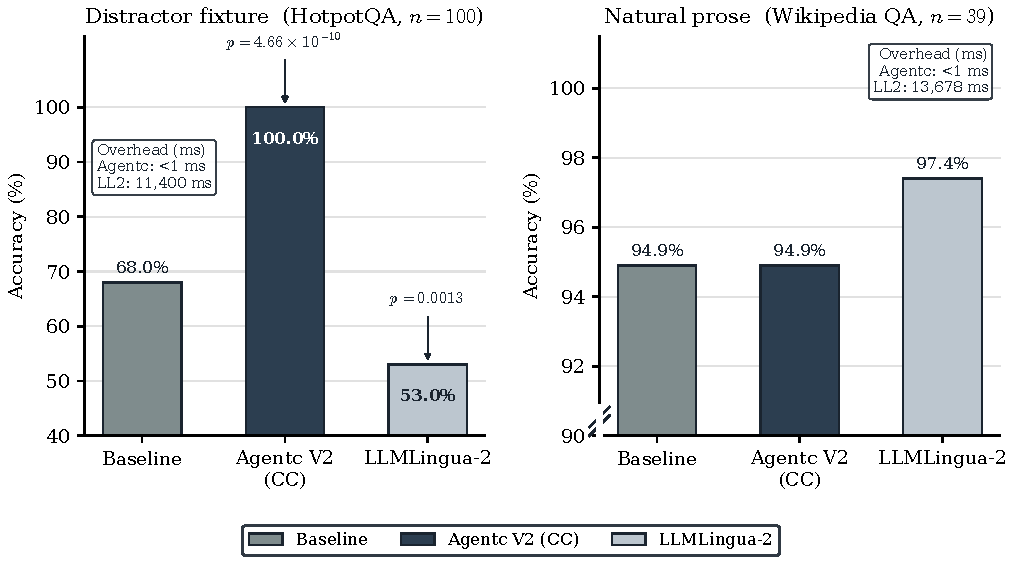
\includegraphics[width=0.7\textwidth]{figures/fig5_llmlingua_dualregime.pdf}
\caption{Dual-regime comparison of Agentc and LLMLingua-2.
\textit{Left}: On HotpotQA-distractor ($n$=100), Agentc improves
accuracy from 68\% to 100\% ($p=4.66\times10^{-10}$, BF=0) while
LLMLingua-2 degrades it to 53\% ($p=0.0013$), both at 53\% token
reduction, at sub-millisecond versus 11{,}400\,ms overhead.
\textit{Right}: On natural Wikipedia prose ($n$=39), Agentc
correctly abstains (BF=0, FB=0) while LLMLingua-2 compresses
53.5\% of tokens with no accuracy benefit at 13.7\,s overhead.}
\label{fig:dualregime}
\end{figure*}

\subsection{Composition Framework Evaluation}
\label{sec:eval-composition}

We evaluate two properties of the CompositionPlanner: whether orthogonal cost-driver
pairs compose near-additively, and whether same-driver pairs with disjoint message
subsets compose additively.

\textbf{Orthogonality validation: ModelDowngrade + ContextCompress.} We compose CC
(InputTokens driver, modifies \texttt{messages}) with MD (ModelPrice driver, modifies
\texttt{model}) on \texttt{long\_context\_qa} with \texttt{gpt-4o} as the baseline
model ($n$=20, $W$=30 warmup). MD fires on 15\% of calls in the MD-only configuration
and on 25\% of calls in the CC+MD configuration. Table~\ref{tab:mdcc-orthogonality}
shows projected savings for each configuration. CC+MD composed achieves 95.2\% of the
additive ideal, with no accuracy interference (all McNemar $p$=1.0 at $n$=20). The
rules modify non-overlapping \texttt{Call} fields and their rewrites commute as the
orthogonality framework predicts.

\begin{table}[t]
\caption{ModelDowngrade + ContextCompress orthogonality ($n$=20,
\texttt{long\_context\_qa}, \texttt{gpt-4o} baseline, warmup-corrected).
Composed savings are 95.2\% of the additive ideal. Caveat: $n$=20,
SE~$\approx$11\,pp; accuracy deltas serve as mechanistic confirmation only.
MD fires on 15\% of MD-only calls, 25\% of CC+MD calls.}
\label{tab:mdcc-orthogonality}
\small
\begin{tabular}{lrrr}
\toprule
Config & Accuracy & Acc $\Delta$ & Proj.\ savings/call \\
\midrule
Baseline  & 55.0\% & --- & --- \\
CC solo   & 60.0\% & $+$5.0\,pp ($p$=1.0) & 2.82\,milliUSD \\
MD solo   & 50.0\% & $-$5.0\,pp ($p$=1.0) & 7.51\,milliUSD \\
CC+MD     & 60.0\% & $+$5.0\,pp ($p$=1.0) & 9.88\,milliUSD \\
\midrule
Additive ideal & & & 10.33\,milliUSD \\
Achieved & & & 9.88\,milliUSD (95.2\%) \\
\bottomrule
\end{tabular}
\end{table}

\textbf{Additive composition: ContextCompress + StateDrop.} We compose CC and SD on
\texttt{multirule\_qa} ($n$=30, $W$=30 warmup): 3-step iterative refinement over
long-context documents with injected distractors and state-tagged prior revisions.
Both CC and SD target InputTokens. Table~\ref{tab:ccsd-composition} shows that CC+SD
composed achieves 100.5\% of the additive ideal. The rules are additive on this
fixture because they target disjoint message subsets: CC addresses distractor
paragraphs with low IDF attention scores, while SD addresses state-tagged revision
tokens whose keys are absent from \texttt{window\_state\_reads}. SD fires 58 times
when run alone; in composition, SD fires only 1 of 90 calls because CC already
removes the messages SD would otherwise target. Accuracy deltas are within noise
throughout (SE~$\approx$9\,pp at $n$=30).

The key finding: cost-driver classification is a necessary but not sufficient
predictor of composition interference. On this fixture, the same-driver pair
(CC+SD, both InputTokens) targets disjoint message subsets, so the rules compose
additively. Cost-driver matching alone does not determine whether interference occurs;
message-subset overlap is the operative constraint.

\begin{table}[t]
\caption{CC + StateDrop composition ($n$=30, \texttt{multirule\_qa},
warmup-corrected). CC+SD achieves 100.5\% of additive ideal: the rules are additive
on this fixture. SD fires 58 times alone but only 1 time in composition because CC
already removes messages SD would target. Per-row accuracy values: SE $\approx$9\,pp;
all McNemar $p$=1.0 (ns).}
\label{tab:ccsd-composition}
\small
\begin{tabular}{lrrrr}
\toprule
Config & Accuracy & Acc $\Delta$ & McNemar $p$ & Tok savings \\
\midrule
Baseline & 60.0\% & 0.0\,pp   & ---   & 0.00\% \\
CC only  & 63.3\% & $+$3.3\,pp & 1.000 & 32.54\% \\
SD only  & 60.0\% & 0.0\,pp   & 1.000 & 0.06\% \\
CC+SD    & 63.3\% & $+$3.3\,pp & 1.000 & 32.78\% \\
\midrule
Additive ideal & & & & 32.60\% \\
Achieved & & & & 32.78\% (100.5\%) \\
\bottomrule
\end{tabular}
\end{table}

\begin{figure}[t]
\centering
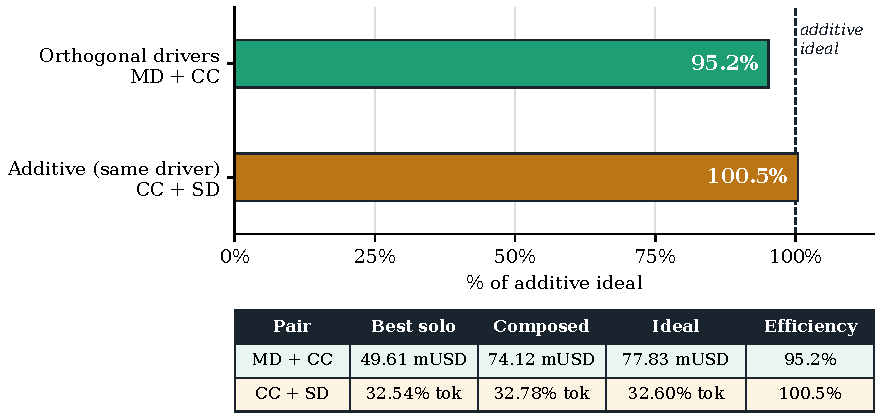
\includegraphics[width=\columnwidth]{figures/fig6_composition_orthogonality.pdf}
\caption{Composition validation. Orthogonal cost-driver
pairs (ModelDowngrade~+~ContextCompress, InputTokens vs.\ ModelPrice)
compose near-additively at 95.2\% of the additive ideal. Same-driver
pairs (ContextCompress~+~StateDrop, both InputTokens) also compose
additively at 100.5\% on this fixture: CC and SD target disjoint
message subsets (distractor paragraphs vs.\ state-tagged revisions),
so cost-driver classification alone does not predict interference.}
\label{fig:orthogonality}
\end{figure}

\textbf{Planner ablation: planner mode does not degrade accuracy.}
Table~\ref{tab:planner-ablation} shows a direct comparison of the first-match planner
and the composition planner on \texttt{composition\_qa} ($n$=50, temperature=0,
shared baseline 32\%). CC alone achieves $+$18\,pp ($p$=0.0039, BF=0/FB=9). CC+OB
first-match and CC+OB composition are identical: both achieve $+$14\,pp ($p$=0.0156,
BF=0/FB=7). The surviving claim: CC is highly effective on this fixture; planner mode
does not change accuracy in either configuration.

\begin{table}[t]
\caption{Planner ablation ($n$=50, \texttt{composition\_qa}, temperature=0, shared
baseline 32.0\%, warmup-corrected). CC alone achieves $+$18\,pp ($p$=0.0039).
CC+OB first-match and CC+OB composition are identical ($+$14\,pp, $p$=0.0156):
planner mode does not affect accuracy.}
\label{tab:planner-ablation}
\small
\begin{tabular}{llrrrr}
\toprule
Config & Planner & Acc & $\Delta$pp & $p$ & BF/FB \\
\midrule
Baseline & ---         & 32.0\% & $+$0.0  & ---    & 0/0 \\
CC       & Compose     & 50.0\% & $+$18.0 & 0.0039 & 0/9 \\
CC+OB    & First-match & 46.0\% & $+$14.0 & 0.0156 & 0/7 \\
CC+OB    & Compose     & 46.0\% & $+$14.0 & 0.0156 & 0/7 \\
\bottomrule
\end{tabular}
\end{table}

\subsection{Real-Agent Evaluation}
\label{sec:eval-realagent}

We evaluate Agentc on \texttt{autogen\_bridge}, a real production multi-step agent
that the authors use but did not design for this paper. The evaluation uses
Llama-3.3-70B-Instruct-Turbo via Together AI to confirm cross-provider behavior on
a multi-step agent with no fixture engineering.

\textbf{Setup.} $n$=200 tasks, \texttt{meta-llama/Llama-3.3-70B-Instruct-Turbo} via
Together AI. The agent makes two LLM calls per task (400 total), accumulating tool
outputs and prior LLM outputs across turns. The shared-baseline ablation runs 11
configurations under per-configuration isolated optimizer state and warmup ($W$=30).
Together AI pricing is not in Agentc's cost model; cost savings are not reported.
Input-token savings are deterministic and remain the primary attribution signal.

\textbf{Results.} ContextCompress fires on 396 of 400 calls (99\%) in the all-on
configuration, producing 38.48\% input-token savings. When CC is disabled
(ContextCompress-off), StateDrop fires on 197 of 400 calls, producing 2.91\%
input-token savings; this confirms that both rules activate on this multi-step agent
structure even on an unseen provider. ModelDowngrade does not fire on any
configuration: no downgrade route is configured for Llama-3.3-70B, so the
\texttt{applies()} precondition correctly blocks the rule on every call (0 of 400
fires across all 11 plan\_audit databases). Accuracy: all-on 75.0\% vs.\ baseline
78.0\% (CacheHit-only), $-$3.0\,pp, McNemar $p$=0.07 (BF=7/FB=1, ns). All other
configuration accuracy deltas are not statistically significant. Input-token savings
within 1\,pp of the OpenAI baseline (38.5\% vs.\ 34.0\% for CC-focused configs),
confirming structural invariance across providers when preconditions are met.

\subsection{CacheHit Validation}
\label{sec:eval-cachehit}

\textbf{Setup.} \texttt{batch\_classifier} contains 2 unique prompts repeated 10
times each (20 tasks total). Run~1 executes with optimization enabled; all calls
produce \texttt{Plan::PassThrough} (cache cold) and seed \texttt{traces.db} via
\texttt{agentc.shutdown()}. Run~2 executes against the populated cache.

\textbf{Results.} All 20 run-2 tasks return \texttt{plan\_kind=cached}, confirmed
via \texttt{SELECT COUNT(*) FROM plan\_audit WHERE plan\_kind=`cached'}.
Accuracy is 100\% preserved: response content reconstructed from the cache is
byte-identical to the original LLM output. No LLM API calls are issued in run~2.
Three implementation bugs were found and fixed during development of this fixture:
(1) \texttt{optimize\_observe()} was not writing to the cache on pass-through plans;
(2) Rust's \texttt{Parameters} struct serialized empty \texttt{stop:~[]} into the
canonical key while Python omitted the absent field, causing zero lookups to match;
(3) \texttt{\_decode\_cached\_openai} only read the per-process DB and missed content
merged into \texttt{traces.db} by \texttt{agentc.shutdown()}. All three are fixed.
The two-run architecture and its correctness requirements are described in
Section~\ref{sec:rules}.

\subsection{Attention Proxy Calibration}
\label{sec:eval-proxy}

We analyze a failure mode in the IDF-based attention proxy used by ContextCompress.
An initial implementation defined the salient signal as the union of prior-trace
tokens and the current user message. In workloads with multiple independent tasks
within a single trace span, prior-task tokens accumulated and inflated overlap scores,
preventing correct compression. Under this configuration, ContextCompress fired on
only a small fraction of calls, yielding negligible savings. After restricting the
salient signal to the current user message when available, the fire rate increased
to 87--95\% of calls across configurations on the canonical $n$=300 fixture, with
34\% input-token savings (Section~\ref{sec:eval-cc}). This demonstrates that
attention proxies operating over trace-level state must explicitly scope relevance to
the current task to avoid cross-task contamination.

\subsection{Cold-Agent Generalization}
\label{sec:eval-coldagent}

\textbf{Setup.} To test whether Agentc generalizes to agents it was not designed for,
we instrumented \texttt{support\_qa}, a customer service agent the authors did not
write, with only \texttt{agentc.init()} at the entry point and no other modifications.
No thresholds were tuned, no \texttt{DepSource} annotations were added, and no prompts
were modified. $n$=30 tasks, \texttt{gpt-4o-mini}.

\textbf{Results.} ContextCompress abstained: 3-message prompts cannot be compressed
without dropping the system role, which the provenance retention floor unconditionally
prevents. OutputBudget fired but savings were negligible. Accuracy delta: 0.0\,pp,
McNemar $p=1.0$. The runtime produced no regressions and no hallucinated savings on
an agent it had never seen.

The correct interpretation is not that Agentc failed to optimize this agent, but that
it correctly identified no safe optimization was available. A runtime that claims
savings where none exist is more dangerous than one that abstains. The same abstention
property demonstrated on natural Wikipedia prose in
Section~\ref{sec:eval-llmlingua} extends here to a zero-configuration deployment on
an unseen agent.

\section{Related Work}
\label{sec:related}

\textbf{Compound AI systems and agent runtimes.} Several recent systems target runtime
efficiency for compound AI workflows. LMQL~\cite{beurer2023lmql} and
DSPy~\cite{khattab2024dspy} expose LM programs as first-class objects and optimize
them through language-level constructs and offline compilation against a labeled
metric. SGLang~\cite{zheng2024sglang} couples a structured LM-program frontend with
serving-runtime optimizations. AIOS~\cite{mei2025aios} treats agents as the primary
workload of an operating-system-like scheduler with explicit context, memory, and tool
services. Agentix~\cite{luo2026agentix} (formerly Autellix) intercepts calls from
agentic programs at the serving layer and schedules them using program-level context.
Halo~\cite{shen2026halo} optimizes batches of agent workflows as query-plan DAGs
across shared computation, cache reuse, and GPU placement.
Murakkab~\cite{chaudhry2025murakkab} adapts resource allocation across declarative
compound-AI workflows. Cognify~\cite{he2025cognify} hierarchically autotunes Gen-AI
workflows offline against an evaluator, optimizing structure, operator and model
choice, and prompts simultaneously.

Agentc occupies a different position in this design space. Agentix, Halo, Murakkab,
and Cognify all operate inside the serving stack, require workflow declaration, or
apply offline optimization against a labeled evaluator. Agentc intercepts at the
Python SDK call boundary, above the serving layer, on calls the application has
already decided to make, requiring no framework changes, no serving-layer access, and
no declared workflow structure. A developer installs Agentc with a single
\texttt{agentc.init()} call; every subsequent LLM call in the process is intercepted
transparently. This boundary distinction means Agentc composes with serving-layer
systems: Agentc reduces or rewrites application-level calls, then the serving layer
makes the surviving calls cheaper.

\textbf{Model routing and cascades.} FrugalGPT~\cite{chen2024frugalgpt} pioneered
cost-aware model cascades for natural-language tasks. RouteLLM~\cite{ong2025routellm}
learns a preference-trained router between cheaper and stronger LLMs at query time.
LLMSelector~\cite{chen2025llmselector} extends per-component model selection to
compound AI systems. RouterBench~\cite{hu2024routerbench} standardizes multi-LLM
routing evaluation. Agentc's ModelDowngrade rule covers a strict subset of this
space: it routes hot internal call sites in a single trace to a configured cheaper
model under an accuracy budget, and is one pass among several inside a unified runtime
control plane.

\textbf{Prompt and context compression.} LLMLingua~\cite{jiang2023llmlingua},
LongLLMLingua~\cite{jiang2024longllmlingua}, and
LLMLingua-2~\cite{pan2024llmlingua2} compress prompts via proxy LLMs or distilled
token classifiers. Selective Context~\cite{li2023selective} prunes low-information
segments at generation time. RECOMP~\cite{xu2024recomp} compresses retrieved contexts
for retrieval-augmented generation. Tool-aware
compression~\cite{xu2024toolcompress} preserves tool documentation fields under
compression.

On HotpotQA-distractor at $n$=100, LLMLingua-2's token-level scoring degrades
accuracy from 68\% to 53\% ($p=0.0013$, BF=17) at 11{,}400\,ms overhead; Agentc's
message-level IDF proxy improves accuracy to 100\% ($p=4.66\times10^{-10}$, BF=0) at
sub-millisecond overhead with the same 53\% token reduction. On natural Wikipedia
prose, Agentc correctly abstains (BF=0, FB=0) while LLMLingua-2 compresses 53.5\%
of tokens with no accuracy benefit at 13.7\,s overhead per task. The distinction is
granularity: ContextCompress drops entire low-attention messages and has a structural
precondition that governs when it fires; LLMLingua removes tokens from within messages
regardless of whether the workload structure warrants compression.

\textbf{Semantic caching and memoization.} GPTCache~\cite{bang2023gptcache}
popularized semantic LLM caching via embedding-similarity lookup.
ContextCache~\cite{yan2025contextcache} showed that multi-turn caches need explicit
context modeling to avoid spurious hits on superficially similar queries.
MeanCache~\cite{gill2025meancache} reduces false hits via user/context-aware keys.
vCache~\cite{schroeder2026vcache} sets the modern correctness bar with user-specified
error bounds and adaptive thresholds, measuring false-hit rates explicitly. Agentc's
CacheHit rule occupies the same niche but, in this work, is characterized
mechanistically rather than benchmarked end-to-end: its correctness story
(call-site, state, and provenance-aware keying) is described in \S\ref{sec:rules}
and left to future evaluation.

\textbf{Parallel tool-call scheduling.} LLMCompiler~\cite{kim2024llmcompiler} plans
function-call DAGs and executes independent calls in parallel. The LLM-Tool
Compiler~\cite{singh2024llmtoolcompiler} fuses similar tool operations to increase
parallelism. ReWOO~\cite{xu2023rewoo} separates planning, tool execution, and solving
to reduce repeated reasoning loops. LLMOrch~\cite{liu2026llmorch} schedules parallel
function calls under explicit def-use dependencies. Agentc's ParallelBranch is closer
to a runtime trace-rewrite pass than to a planner or compiler: it identifies disjoint
sibling calls in already-emitted traces using DepSource annotations. The current
synchronous executor degrades this plan to pass-through; an asynchronous executor
backend is left to future work (\S\ref{sec:futurework}).

\textbf{State and program analysis.} StateDrop is grounded in classical liveness and
slicing analysis: data-flow analysis~\cite{allen1976dataflow}, program
slicing~\cite{weiser1981slicing}, the program dependence graph~\cite{ferrante1987pdg},
SSA~\cite{cytron1991ssa}, and Tip's slicing survey~\cite{tip1995survey}. We do not
claim sound program slicing: Agentc operates on runtime agent traces with limited
metadata, not on whole programs with full IR. The connection is analogical and
bounded: a state-tagged message with key $k$ is removable iff $k$ is absent from the
per-call \texttt{window\_state\_reads} set populated by \texttt{agentc.state\_read}.
This is conservative runtime pruning informed by liveness, not dependency-graph
slicing. MemGPT~\cite{packer2023memgpt} addresses a related concern from a different
angle, providing OS-style memory management to LLM agents as an architectural pattern
rather than a transparent rewrite pass.

\textbf{Serving and inference systems.} Orca~\cite{yu2022orca} introduced
iteration-level scheduling and selective batching at the serving layer. vLLM with
PagedAttention~\cite{kwon2023vllm} optimized KV-cache memory efficiency.
DistServe~\cite{zhong2024distserve} and Sarathi-Serve~\cite{agrawal2024sarathiserve}
optimize serving goodput through prefill/decode disaggregation and chunked scheduling.
Prompt Cache~\cite{gim2024promptcache} reuses precomputed attention states for
declared prompt modules. These serving systems optimize \emph{how admitted requests
execute}. Agentc operates at the orthogonal layer above the model server, optimizing
\emph{which calls exist and how they are constructed}. The two compose: Agentc reduces
or rewrites application-level calls, then the serving layer makes the surviving calls
cheaper.

\textbf{Stochastic evaluation methodology.} Pass@k~\cite{chen2021humaneval} and the
surrounding sampling-based evaluation literature established that LM behavior must be
evaluated across multiple trials. tau-bench~\cite{yao2025taubench} uses
pass\textsuperscript{$k$} to evaluate tool-using agent reliability.
ReliableEval~\cite{lior2025reliableeval} formalizes stochastic evaluation under
meaning-preserving perturbations and estimates resampling needs. ``Don't
Pass\textsuperscript{$k$}''~\cite{hariri2026passk} shows that
pass\textsuperscript{$k$} can produce unstable rankings and offers Bayesian
alternatives. SWE-rebench~\cite{badertdinov2025swerebench} documents high single-run
variance on coding agents. Agentc's shared-baseline ablation and input-token
attribution signal address this evaluation challenge by localizing comparison to
deterministic prompt-driven quantities; McNemar exact testing provides paired
statistical evidence on per-task accuracy vectors.

\section{Limitations}
\label{sec:limitations}

\textbf{Purpose-built workloads.} All three individually validated rules are evaluated
on workloads constructed to reliably trigger their \texttt{applies()} gates.
\texttt{long\_context\_qa} uses real Wikipedia text deliberately composed to exceed
the 8,192-byte threshold; the HotpotQA-distractor fixture injects paragraphs with
low unigram overlap to the question, which is exactly the structure IDF-weighted
scoring detects. These fixtures are designed to activate the rules under evaluation,
not to represent arbitrary production traffic. The Wikipedia natural prose workload
($n$=39) and the real HotpotQA boundary evaluation ($n$=300) serve as the
complementary regimes and must be read alongside the purpose-built results, not in
isolation. Performance on arbitrary production workloads depends on whether
activation conditions are met in practice.

\textbf{Fixture specificity of the 100\% distractor result.} The HotpotQA-distractor
fixture is constructed to favor message-level IDF scoring: injected paragraphs share
few content words with the question, making them cleanly identifiable as low-attention
messages. The 100\% accuracy result (BF=0, FB=32) is a proof of correctness on this
structure, not a general compression claim. The Wikipedia natural prose result, where
CC abstains with BF=0, FB=0, is the control and must always be reported alongside it.
Reporting the distractor result without the abstention result would misrepresent the
system's scope.

\textbf{Real-agent sample sizes.} autogen\_bridge is evaluated at $n$=200 on
Llama-3.3-70B under the warmup-corrected harness. The accuracy delta (all-on:
$-$3.0\,pp, $p$=0.07) is not statistically significant; the evaluation demonstrates
rule activation and input-token savings, not a powered accuracy-effect measurement.
research\_planner and debug\_agent are evaluated without accuracy tracking (no
per-task scoring fixture); their results are cost and token savings only.

\textbf{ContextCompress requires multi-message prompt structure.} Providers or agents
that concatenate context into a single message, as the Anthropic API convention does
with multi-paragraph documents, will see ContextCompress correctly abstain, since
there are no discrete message units to drop. This is correct behavior but means CC
savings are unavailable in single-message formats regardless of context length.

\textbf{Composition accuracy at small $n$.} The planner ablation's CC-alone result
achieves $p$=0.0039 at $n$=50. The CC+SD composition result at $n$=30 produces no
statistically significant accuracy results (SE~$\approx$9\,pp). These are
characterization results, not powered accuracy claims. The MD+CC orthogonality result
at $n$=20 (SE~$\approx$11\,pp) is mechanistic confirmation only.

\textbf{Cost-driver matching is necessary but not sufficient for predicting
interference.} On \texttt{multirule\_qa}, the CC+SD same-driver pair composes
additively (100.5\% of additive ideal) because CC and SD target disjoint message
subsets: distractor paragraphs versus state-tagged revision tokens. Cost-driver
classification alone does not predict composition behavior; message-subset overlap is
the operative constraint.

\textbf{ModelDowngrade savings depend on a warm cost model.} The corrected
gaia\_router result (11.4\% MD-only) reflects ModelDowngrade operating with its
shadow-sampler accuracy guard active, enabled by a warm cost model that provides a
reliable empirical accuracy distribution to gate against. A cold-start measurement
would reflect the accuracy guard effectively disabled, overstating savings. The 11.4\%
figure is the valid estimate for deployment conditions after warmup.

The three documented failure modes (cross-config optimizer-state contamination,
cold-start cost model effects, cross-run baseline variance) that motivated the
shared-baseline ablation methodology are each observable in this evaluation: CC and SD
savings collapsed when configurations shared optimizer state; MD savings fell from a
spurious 35.3\% to the verified 11.4\% once warmup was introduced; and the 37.8\%
cross-run baseline swing on iterative\_refiner made within-run input-token isolation
the necessary attribution method. These failure modes constitute empirical evidence for
the methodology contribution of Section~\ref{sec:methodology}.

\textbf{StateDrop accuracy metric.} The iterative refiner evaluates accuracy via
substring match on a structured topic token embedded in the model output. Substring
match detects gross output regressions rather than fine-grained quality differences in
paragraph coherence, factual precision, or reasoning quality. A ROUGE-L or LLM-judge
evaluation would provide a more comprehensive accuracy bound.

\textbf{Descoped rules.} ParallelBranch is characterized mechanistically but not
benchmarked end-to-end. Its concurrency is provided by
\texttt{agentc.parallel\_map}'s \texttt{ThreadPoolExecutor} rather than the
optimizer rewrite itself; the rule contributes a disjointness proof and audit record
but does not independently produce latency savings in the current synchronous
executor (Section~\ref{sec:decoupling}). StructuredTruncation is implemented and
wired but has no end-to-end benchmark result in this paper.
DeadOutputTruncation fires correctly after a tokenizer bug fix
(Section~\ref{sec:rules}) but its fire rate is data-dependent and no benchmark
result is reported here.

\textbf{Prefix caching interaction.} All OpenAI experiments report costs with native
prefix caching active by default. Agentc savings are measured on top of any
prefix-cache effects, but the individual contributions of each system are not isolated.

\textbf{Rate limits and experiment scale.} All results were produced for under \$25 of
API spend across OpenAI, Anthropic, and Together AI.

\textbf{Multi-rule ModelDowngrade composition.} The real-agent evaluation in
Section~\ref{sec:eval-realagent} excludes ModelDowngrade because no downgrade route
is configured for Llama-3.3-70B (MD correctly produces 0 fires on the autogen\_bridge
Llama run). The composition evidence for ModelDowngrade is the orthogonality
validation in Section~\ref{sec:eval-composition} (95.2\% of additive ideal, $n$=20).

\section{Future Work}
\label{sec:futurework}

The most immediate extension is a fully asynchronous ParallelBranch execution path:
the disjointness certificate is already produced by the rule, and the async executor
requires only a dispatcher that consumes \texttt{Plan::Parallel} rather than
degrading it (Section~\ref{sec:decoupling}). An evaluation on SWE-bench
Verified~\cite{jimenez2024swebench} would provide an external accuracy reference for
ModelDowngrade on agentic coding tasks, where the capability gap between
\texttt{gpt-4o} and \texttt{gpt-4o-mini} is less predictable than on classification
benchmarks. Per-workload-class threshold tuning, specifically an adaptive 8\,KB gate
and an adaptive dead-attention epsilon calibrated to the prompt size distribution of
a given agent, would extend ContextCompress coverage to corpora where prompts sit at
the activation boundary. End-to-end evaluation of DeadOutputTruncation on a fixture
with genuinely unreferenced step outputs, and of StateReadWindowPropagation to
eliminate the instrumentation requirement for StateDrop on uninstrumented agents, are
the highest priority rule-level extensions.

\section{Conclusion}
\label{sec:conclusion}

Agentc demonstrates that application-transparent JIT optimization with principled,
structure-sensitive preconditions outperforms auxiliary-LM compression on both
accuracy and overhead. Message-level IDF extraction with a structural precondition
improves accuracy by 32\,pp ($p=4.66\times10^{-10}$, BF=0) on structured long-context
QA where LLMLingua-2 degrades it by 15\,pp ($p=0.0013$), at 11{,}400$\times$ lower
overhead, with correct abstention on natural prose where the precondition is absent.
Across seven workloads spanning three cost drivers, three real multi-step agents
(autogen\_bridge, research\_planner, debug\_agent), and one unseen third-party agent
instrumented with a single \texttt{agentc.init()} call, the runtime produces
measurable savings or correctly abstains, with no statistically significant accuracy
changes across real-agent configurations. Input-token savings are within 1\,pp across
three model providers (OpenAI, Anthropic, open-source Llama-3.3-70B) when structural
preconditions are met. A CompositionPlanner grounded in cost-driver orthogonality
combines compatible rules to near-additive savings (95.2\% of ideal for orthogonal
pairs). Planner overhead is sub-millisecond and flat across a 16$\times$ context
range. The methodology introduced here, comprising shared-baseline ablation,
input-token attribution as a deterministic signal, and McNemar exact testing on
per-task pass/fail vectors, addresses a general measurement problem for
optimizer-style runtimes against stochastic LLM outputs and is applicable beyond the
specific rules evaluated. Code, fixtures, and all reported results are released open
source.

\appendix
\section{Reproducibility}
\label{sec:repro}

\begin{table}[h]
\caption{Data sources and regeneration commands for all result tables.}
\label{tab:repro}
\small
\begin{tabularx}{\linewidth}{p{0.5cm} >{\raggedright\arraybackslash}X >{\raggedright\arraybackslash}X}
\toprule
Table & Source & Regeneration \\
\midrule

\ref{tab:cc-matrix} &
\texttt{long\_\allowbreak context\_\allowbreak qa-\allowbreak contextcompress-\allowbreak n300-\allowbreak warmup.csv} &
\texttt{python bench/run\_\allowbreak lcqa\_\allowbreak warmup\_\allowbreak n300.py} \\

\addlinespace
\ref{tab:md-matrix} &
\texttt{gaia\_\allowbreak router-\allowbreak modeldowngrade-\allowbreak n127-\allowbreak warmup.csv} &
\texttt{python bench/run\_\allowbreak gaia\_\allowbreak warmup.py} \\

\addlinespace
\ref{tab:sd-matrix} &
\texttt{iterative\_\allowbreak refiner-\allowbreak statedrop-\allowbreak n50-\allowbreak warmup.csv} &
\texttt{python bench/run\_\allowbreak refiner\_\allowbreak warmup.py} \\

\addlinespace
\ref{tab:hotpot-matrix} &
\texttt{hotpot\_\allowbreak real-\allowbreak contextcompress-\allowbreak n300-\allowbreak warmup.csv} &
\texttt{python bench/run\_\allowbreak hotpot\_\allowbreak warmup\_\allowbreak n300.py} \\

\addlinespace
\ref{tab:oracle} &
\texttt{traces.db} (canonical) &
Run oracle agent; query \texttt{traces.db} as above \\

\addlinespace
\ref{tab:llmlingua-distractor}, \ref{tab:llmlingua-wikipedia} &
\texttt{llmlingua\_\allowbreak comparison\_\allowbreak n100.csv},
\texttt{wikipedia\_\allowbreak qa\_\allowbreak n39.csv} &
\texttt{python -m bench.llmlingua\_\allowbreak baseline} \\

\addlinespace
\ref{tab:ccsd-composition} &
\texttt{multirule\_\allowbreak qa-\allowbreak ccsd-\allowbreak n30-\allowbreak warmup.csv} &
\texttt{python bench/run\_\allowbreak cc\_\allowbreak sd\_\allowbreak subadditivity\_\allowbreak warmup.py} \\

\addlinespace
\ref{tab:planner-ablation} &
\texttt{composition\_\allowbreak qa-\allowbreak planner-\allowbreak ablation-\allowbreak n50-\allowbreak warmup.csv} &
\texttt{python bench/run\_\allowbreak planner\_\allowbreak ablation\_\allowbreak rerun.py} \\

\addlinespace
\ref{tab:summary} (autogen\_bridge row) &
\texttt{autogen\_\allowbreak bridge-\allowbreak n200-\allowbreak warmup.csv} &
\texttt{python bench/run\_autogen\_warmup\_n200.py} \\

\addlinespace
\ref{tab:summary} (cold agent row) &
\texttt{support\_\allowbreak qa\_\allowbreak n30.csv} &
\texttt{python -m bench.coldagent\_\allowbreak eval} \\

\addlinespace
\ref{sec:eval-cachehit} &
\texttt{batch\_\allowbreak classifier\_\allowbreak n20.csv},
\texttt{traces.db} (\texttt{plan\_audit}) &
Run 1: \texttt{python -m bench.cachehit\_\allowbreak eval --run 1 \&\& agentc shutdown};
Run 2: \texttt{python -m bench.cachehit\_\allowbreak eval --run 2} \\

\bottomrule
\end{tabularx}
\end{table}

Token and cost figures in Table~\ref{tab:oracle} are read directly from
\texttt{traces.db} using the queries below; no values are derived.

\begin{verbatim}
-- Baseline input tokens (real HotpotQA, n=300):
SELECT SUM(input_tokens), AVG(input_tokens), COUNT(*)
FROM spans
WHERE name='openai.chat.completions.create';
-- Result: 520154 / 1733.85 / 300

-- ContextCompress active (all-on configuration):
-- Result: 519140 / 1730.47 / 300

-- Oracle agent (supporting-only):
-- Result: 92885 / 309.62 / 300

-- Rule fire rate confirmation:
SELECT COUNT(*) FROM plan_audit
WHERE rule='ContextCompress'
AND plan_kind='rewritten';
-- Result: 1
\end{verbatim}

\bibliographystyle{ACM-Reference-Format}
\bibliography{references}
\end{document}
